\documentclass[symmetric, justified, a4paper]{tufte-book}

%% configuration, packages

% Switch this variable true/false to print or hide lecturer notes.
\newcommand{\printlecnotes}{true}

\usepackage{colortbl} 

\hypersetup{colorlinks}% uncomment this line if you prefer colored hyperlinks (e.g., for onscreen viewing)

%% TODO add logic for quasar / orange name change

\usepackage{import}

%%
% If they're installed, use Bergamo and Chantilly from www.fontsite.com.
% They're clones of Bembo and Gill Sans, respectively.
%\IfFileExists{bergamo.sty}{\usepackage[osf]{bergamo}}{}% Bembo
%\IfFileExists{chantill.sty}{\usepackage{chantill}}{}% Gill Sans

%\usepackage{microtype}

\usepackage{tcolorbox}
\usepackage[english]{babel}

%%
% For nicely typeset tabular material
\usepackage{booktabs}

% For stacking images
\usepackage{stackengine}

\usepackage{wrapfig}
\setlength{\wrapoverhang}{5.5cm} % this is something we can set in future to whatever the exact position is

%%
% For graphics / images
\usepackage{graphicx}
%\setkeys{Gin}{width=\linewidth,totalheight=\textheight,keepaspectratio}  % disabled for problems with scale/resolution
\setkeys{Gin}{keepaspectratio}

\graphicspath{{graphics/}}

% The fancyvrb package lets us customize the formatting of verbatim
% environments.  We use a slightly smaller font.
\usepackage{fancyvrb}
\usepackage{hyperref}
\fvset{fontsize=\normalsize}

%%
% Sets the name of the package between Orange compilations
% Always use this instead of directly referring to Orange or Quasar or Oasys, etc.
\newcommand{\mutation}{Orange}
% \newcommand{\mutation}{scOrange}
% \newcommand{\mutation}{Quasar}
\newcommand{\widget}[1]{\textsl{#1}}
\newcommand{\wn}{~cm$^{-1}$}

%%
% Prints argument within hanging parentheses (i.e., parentheses that take
% up no horizontal space).  Useful in tabular environments.
\newcommand{\hangp}[1]{\makebox[0pt][r]{(}#1\makebox[0pt][l]{)}}

%%
% Prints an asterisk that takes up no horizontal space.
% Useful in tabular environments.
\newcommand{\hangstar}{\makebox[0pt][l]{*}}

%%
% Prints a trailing space in a smart way.
\usepackage{xspace}

\newcommand{\TL}{Tufte-\LaTeX\xspace}

% Prints the month name (e.g., January) and the year (e.g., 2008)
\newcommand{\monthyear}{%
  \ifcase\month\or January\or February\or March\or April\or May\or June\or
  July\or August\or September\or October\or November\or
  December\fi\space\number\year
}


% Prints an epigraph and speaker in sans serif, all-caps type.
\newcommand{\openepigraph}[2]{%
  %\sffamily\fontsize{14}{16}\selectfont
  \begin{fullwidth}
  \sffamily\large
  \begin{doublespace}
  \noindent\allcaps{#1}\\% epigraph
  \noindent\allcaps{#2}% author
  \end{doublespace}
  \end{fullwidth}
}

% Inserts a blank page
\newcommand{\blankpage}{\newpage\hbox{}\thispagestyle{empty}\newpage}

\usepackage{units}

% Typesets the font size, leading, and measure in the form of 10/12x26 pc.
\newcommand{\measure}[3]{#1/#2$\times$\unit[#3]{pc}}

% Macros for typesetting the documentation
\newcommand{\hlred}[1]{\textcolor{Maroon}{#1}}% prints in red
\newcommand{\hangleft}[1]{\makebox[0pt][r]{#1}}
\newcommand{\hairsp}{\hspace{1pt}}% hair space
\newcommand{\hquad}{\hskip0.5em\relax}% half quad space
\newcommand{\TODO}{\textcolor{red}{\bf TODO!}\xspace}
\newcommand{\ie}{\textit{i.\hairsp{}e.}\xspace}
\newcommand{\eg}{\textit{e.\hairsp{}g.}\xspace}
\newcommand{\na}{\quad--}% used in tables for N/A cells
\providecommand{\XeLaTeX}{X\lower.5ex\hbox{\kern-0.15em\reflectbox{E}}\kern-0.1em\LaTeX}
\newcommand{\tXeLaTeX}{\XeLaTeX\index{XeLaTeX@\protect\XeLaTeX}}
% \index{\texttt{\textbackslash xyz}@\hangleft{\texttt{\textbackslash}}\texttt{xyz}}
\newcommand{\tuftebs}{\symbol{'134}}% a backslash in tt type in OT1/T1
\newcommand{\doccmdnoindex}[2][]{\texttt{\tuftebs#2}}% command name -- adds backslash automatically (and doesn't add cmd to the index)
\newcommand{\doccmddef}[2][]{%
  \hlred{\texttt{\tuftebs#2}}\label{cmd:#2}%
  \ifthenelse{\isempty{#1}}%
    {% add the command to the index
      \index{#2 command@\protect\hangleft{\texttt{\tuftebs}}\texttt{#2}}% command name
    }%
    {% add the command and package to the index
      \index{#2 command@\protect\hangleft{\texttt{\tuftebs}}\texttt{#2} (\texttt{#1} package)}% command name
      \index{#1 package@\texttt{#1} package}\index{packages!#1@\texttt{#1}}% package name
    }%
}% command name -- adds backslash automatically
\newcommand{\doccmd}[2][]{%
  \texttt{\tuftebs#2}%
  \ifthenelse{\isempty{#1}}%
    {% add the command to the index
      \index{#2 command@\protect\hangleft{\texttt{\tuftebs}}\texttt{#2}}% command name
    }%
    {% add the command and package to the index
      \index{#2 command@\protect\hangleft{\texttt{\tuftebs}}\texttt{#2} (\texttt{#1} package)}% command name
      \index{#1 package@\texttt{#1} package}\index{packages!#1@\texttt{#1}}% package name
    }%
}% command name -- adds backslash automatically
\newcommand{\docopt}[1]{\ensuremath{\langle}\textrm{\textit{#1}}\ensuremath{\rangle}}% optional command argument
\newcommand{\docarg}[1]{\textrm{\textit{#1}}}% (required) command argument
\newenvironment{docspec}{\begin{quotation}\ttfamily\parskip0pt\parindent0pt\ignorespaces}{\end{quotation}}% command specification environment
\newcommand{\docenv}[1]{\texttt{#1}\index{#1 environment@\texttt{#1} environment}\index{environments!#1@\texttt{#1}}}% environment name
\newcommand{\docenvdef}[1]{\hlred{\texttt{#1}}\label{env:#1}\index{#1 environment@\texttt{#1} environment}\index{environments!#1@\texttt{#1}}}% environment name
\newcommand{\docpkg}[1]{\texttt{#1}\index{#1 package@\texttt{#1} package}\index{packages!#1@\texttt{#1}}}% package name
\newcommand{\doccls}[1]{\texttt{#1}}% document class name
\newcommand{\docclsopt}[1]{\texttt{#1}\index{#1 class option@\texttt{#1} class option}\index{class options!#1@\texttt{#1}}}% document class option name
\newcommand{\docclsoptdef}[1]{\hlred{\texttt{#1}}\label{clsopt:#1}\index{#1 class option@\texttt{#1} class option}\index{class options!#1@\texttt{#1}}}% document class option name defined
\newcommand{\docmsg}[2]{\bigskip\begin{fullwidth}\noindent\ttfamily#1\end{fullwidth}\medskip\par\noindent#2}
\newcommand{\docfilehook}[2]{\texttt{#1}\index{file hooks!#2}\index{#1@\texttt{#1}}}
\newcommand{\doccounter}[1]{\texttt{#1}\index{#1 counter@\texttt{#1} counter}}


% do not put empty space before chapters; not needed in this handbook
\titlespacing*{\chapter}{0pt}{0pt}{40pt}

% Allows adding images that go into or over page margins
\newcommand{\infinitewidthbox}[1]{\noindent\makebox[\textwidth]{#1}}

% Generates the index
\usepackage{makeidx}

% Remove "Figure X:" before figures.
% We do not need these in our short chapters.
\usepackage{etoolbox}
\makeatletter
\patchcmd{\@caption}
  {\noindent\csname fnum@#1\endcsname: \ignorespaces}
  {\noindent}
  {}{}
\makeatother

% Do not put additional empty pages before chapters
\makeatletter
\patchcmd{\chapter}{\if@openright\cleardoublepage\else\clearpage\fi}{\clearpage}{}{}
\makeatother


% Lecturer notes
\newtcolorbox{mylecnote}[1][]{%
  size=title,
  boxrule=0.5pt,
  fonttitle={\large\bfseries},
  coltitle={black},
  title={Lecturer note.\ },
  attach title to upper,
  #1
}

\newcommand{\lecnotes}[1]{
	\ifthenelse{\equal{\printlecnotes}{true}}{
	\begin{mylecnote}
		{#1}
	\end{mylecnote}
	}{}
}

%\printnotes{}

\makeindex

%%
% Book metadata
\title{Using \mutation\thanks{Thanks to everyone who worked on this document.}}
\author[Biolab and Collaborators]{Biolab and Collaborators}
\publisher{Biolab}

\begin{document}

% Front matter
\frontmatter

% full title page
\maketitle

% v.4 copyright page
% \iffalse
\newpage
\begin{fullwidth}
~\vfill
\thispagestyle{empty}
\setlength{\parindent}{0pt}
\setlength{\parskip}{\baselineskip}
Copyright \copyright\ \the\year\ \thanklessauthor

\par\smallcaps{Published by \thanklesspublisher}

\par\smallcaps{tufte-latex.googlecode.com}

\par Licensed under the Apache License, Version 2.0 (the ``License''); you may not
use this file except in compliance with the License. You may obtain a copy
of the License at \url{http://www.apache.org/licenses/LICENSE-2.0}. Unless
required by applicable law or agreed to in writing, software distributed
under the License is distributed on an \smallcaps{``AS IS'' BASIS, WITHOUT
WARRANTIES OR CONDITIONS OF ANY KIND}, either express or implied. See the
License for the specific language governing permissions and limitations
under the License.\index{license}

\par\textit{First printing, \monthyear}
\end{fullwidth}

% \fi

\tableofcontents

%\chapter*{Introduction}


\begin{figure*}[t!]
  \includegraphics[width=\linewidth]{graphics/\mutation-intro-fig.jpg}%
  \label{chfig:intro}%
\end{figure*}


\newthought{This book} showcases machine learning and scientific data analysis problems using \mutation\cite{\mutation} through easily reproducible workflows.

First, let us acknowledge that \mutation\ is but a pre-packaged version of Orange\cite{orange} and the Orange Spectroscopy add-on\cite{git\mutation}.

The examples presented here introduce the features of \mutation\ through common data analysis tasks. You will see how common data mining can be accomplished through visual programming. We will also apply the same techniques to spectral data and hyperspectral images. \marginnote{\newthought{These notes include} \mutation\ workflows and visualizations we will construct during the course. 

The original notes were written by the members of the SMIS beam line of the SOLEIL Synchrotron, and the Bioinformatics Lab at University of Ljubljana and are extensions of the notes by Blaž Zupan, Janez Demšar and Marko Toplak.
}
If you are already familiar with data analysis, the methodological aspects of this course will seem simple, but you will have more time to absorb \mutation\ and the \mutation\ philosophy — try to think of what is happening behind the scenes.


\begin{figure*}[b!]
    % \centering
    
\includegraphics[width=30mm]{CC-BY-SA_icon_white.png}
    \label{fig:CC-BY-SA_icon}
\end{figure*}


% Start the main matter (normal chapters)
\mainmatter

%% I would like to have an option of not showing the figure number
%% ? How do we avoid overlapping figure captions?

%%%% ORANGE %%%%

\subimport{chapters/001-workflows/}{workflows}
\subimport{chapters/002-basic-data-exploration/}{basic-data-exploration}
\subimport{chapters/003-saving-your-work/}{saving}
\subimport{chapters/004-loading-data/}{loading-data}
\subimport{chapters/spec-001-spectral-data/}{spectral-data}
\subimport{chapters/spec-010-spectral-pca/}{spectral-pca}
\subimport{chapters/spec-003-hyper-basic/}{hyper-basic}
\subimport{chapters/spec-011-preprocessing/}{spectral-preprocessing}
\subimport{chapters/spec-012-integrals-ratios/}{integrals-ratios}
% Lesson 10: Classification
\chapter{Classification}
\label{ch:classification}

We have seen the iris data before. \marginnote{We call the variable we wish to predict a target variable, or an outcome or, in traditional machine learning terminology, a class. Hence we talk about classification, classifiers, classification trees...} We wanted to predict varieties based on measurements---but we actually did not make any predictions. We observed some potentially interesting relations between the features and the varieties, but have never constructed an actual model.

Let us create one now.

\begin{figure}[h]
    \centering
    \vspace{-0.2cm}
    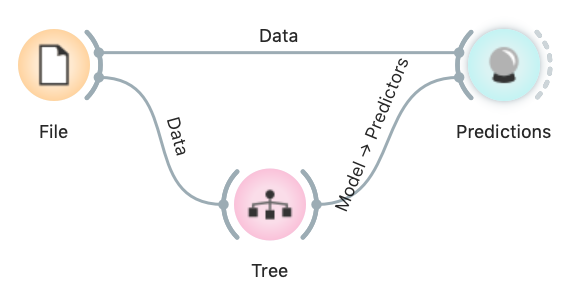
\includegraphics[scale=0.4]{graphics/ch-classification/predictions-workflow.png}
    \caption{Something in this workflow is conceptually wrong. Can you guess what?}
    \label{fig:spectral_preprocessing-fig2}
\end{figure}

\begin{wrapfigure}{o}{1.1\textwidth}
    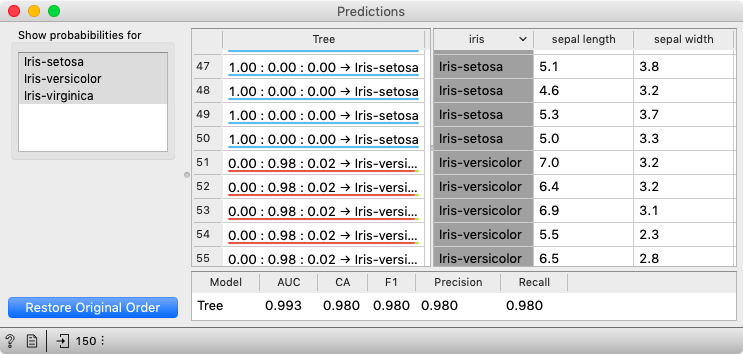
\includegraphics[scale=0.4]{graphics/ch-classification/predictions.png}
    \label{fig:classification-predictions}
\end{wrapfigure}

The data is fed into the Tree widget, which infers a classification model and gives it to the Predictions widget. Note that unlike in our past workflows, in which the communication between widgets included only the data, we here have a channel that carries a predictive model.

The Predictions widget also receives the data from the File widget. The widget uses the model to make predictions about the data and shows them in the table.

How correct are these predictions? Do we have a good model? How can we tell?

But (and even before answering these very important questions), what is a classification tree? And how does Orange create one? Is this algorithm something we should really use?

So many questions to answer!

% Lesson 11: Classification Trees
\chapter{Classification Trees}
\label{ch:classification-trees}

In the previous lesson, we used a classification tree,
\marginnote{Classification trees were hugely popular in the early years of machine learning, when they were first independently proposed by the engineer Ross Quinlan (C4.5) and a group of statisticians (CART), including the father of random forests Leo Brieman.}
one of the oldest, but still popular, machine learning methods. We like it since the method is easy to explain and gives rise to random forests, one of the most accurate machine learning techniques (more on this later). So, what kind of model is a classification tree?

Let us load \textit{iris} data set, build a tree (widget \widget{Tree}) and visualize it in a \widget{Tree Viewer}.

\begin{figure}[h]
    \centering
    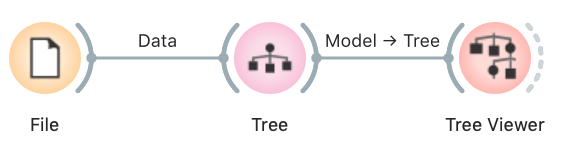
\includegraphics[scale=0.4]{graphics/ch-classification_trees/workflow-tree-viewer.png}
\end{figure}

\begin{figure*}[h]
    \vspace{-0.4cm}
    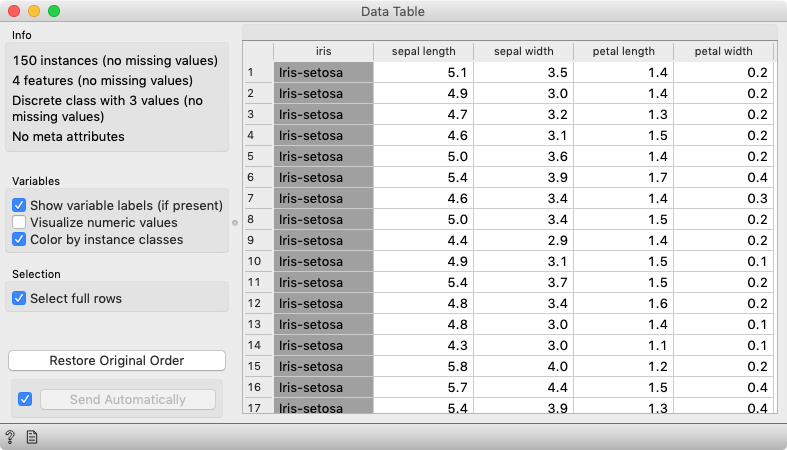
\includegraphics[scale=0.35]{graphics/ch-classification_trees/iris-data.png}
    \label{fig:classification-predictions}
\end{figure*}

\begin{wrapfigure}{o}{1.1\textwidth}
    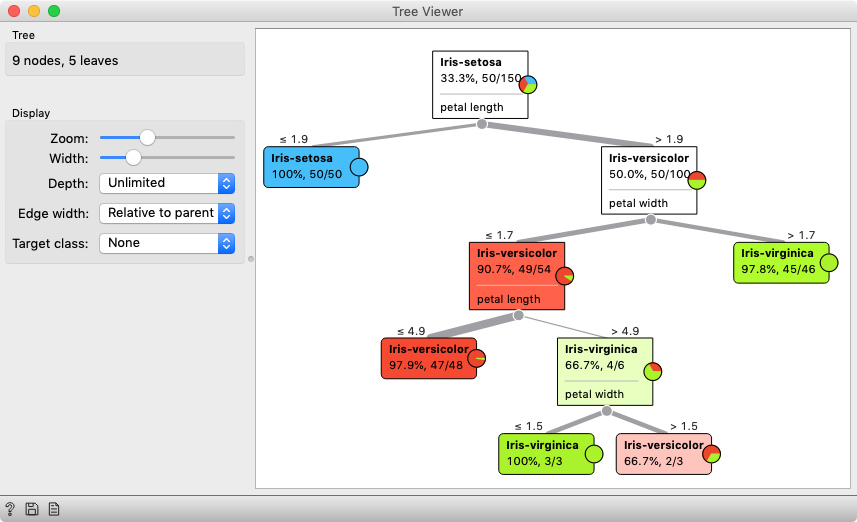
\includegraphics[scale=0.35]{graphics/ch-classification_trees/tree-viewer.png}
    \label{fig:classification-predictions}
\end{wrapfigure}

We read the tree from top to bottom. Looks like the column \textit{petal length} best separates iris variety \textit{setosa} from the others, while \textit{petal width} then almost perfectly separates the remaining two varieties.

Trees place the most useful feature at the root. What would be the most useful feature? The feature that splits the data into two purest possible subsets. It then splits both subsets further, again by their most useful features, and keeps doing so until it reaches subsets in which all data belongs to the same class (leaf nodes in strong blue or red) or until it runs out of data instances to split or out of useful features (the two leaf nodes in white).

We still have not been very explicit about what we mean by ``the most useful'' feature. There are many ways to measure the quality of features, based on how well they distinguish between classes. We will illustrate the general idea with information gain. We can compute this measure in Orange using the \widget{Rank} widget \marginnote{The \widget{Rank} widget can be used on its own to show the best predicting features. Say, to figure out which genes are best predictors of the phenotype in some gene expression data set.}, which estimates the quality of data features and ranks them according to how informative they are about the class. We can either estimate the information gain from the whole data set, or compute it on data corresponding to an internal node of the classification tree in the \widget{Tree Viewer}. In the following example we use the \textit{Sailing} data set.

\begin{figure}[h]
    \centering
    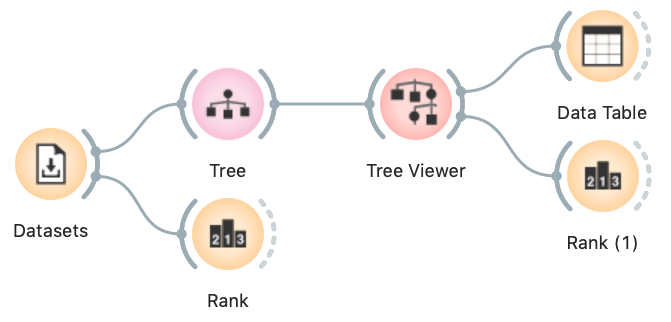
\includegraphics[scale=0.4]{graphics/ch-classification_trees/workflow-rank.png}
    \caption{The \widget{Datasets} widget is set to load the \textit{Sailing} data set. To use the second \widget{Rank}, select a node in the \widget{Tree Viewer}.}
\end{figure}

Besides the information gain, \widget{Rank} displays several other measures (including Gain Ratio and Gini), which are often quite in agreement and were invented to better handle discrete features with many different values.

\begin{figure}[h]
    \centering
    \vspace{-0.2cm}
    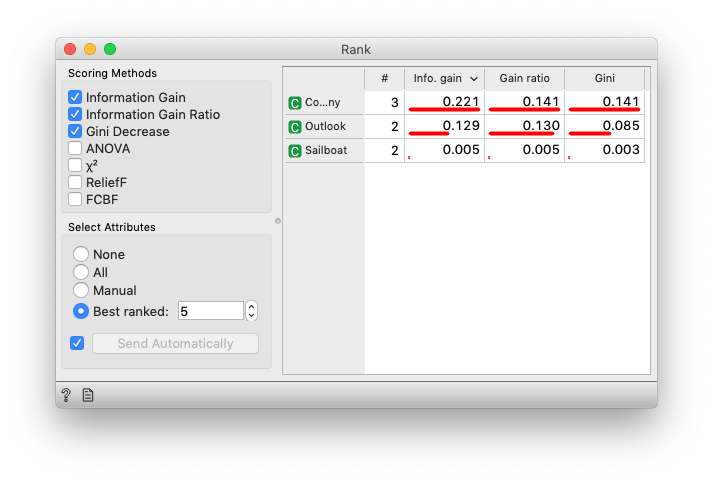
\includegraphics[scale=0.4]{graphics/ch-classification_trees/rank.png}
    \caption{For the whole \textit{Sailing} data set, \textit{Company} is the most class-informative feature according to all measures shown.}
\end{figure}

% Lesson 12: Model Inspection - merged to classification trees
% Lesson 13: Naive Bayes
\chapter{Naive Bayes}
\label{ch:naive_bayes}

Naive Bayes \marginnote{Naive Bayes assumes class-wise independent features. For a data set where features would actually be independent, which rarely happens in practice, the naive Bayes would be the ideal classifier.} is also a classification method. To see how naive Bayes works, we will use a data set on passengers’ survival in the Titanic disaster of 1912. The \textit{Titanic} data set describes 2201 passengers, with their tickets (first, second, thirds class or crew), age and gender.

\begin{figure}[h]
    \centering
    \vspace{-0.2cm}
    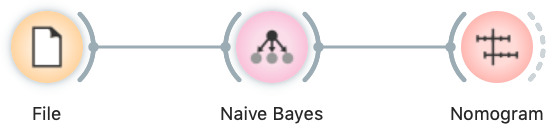
\includegraphics[scale=0.4]{graphics/ch-naive_bayes/workflow.png}
\end{figure}

We inspect naive Bayes models with the \widget{Nomogram} widget. There, we se a scale ‘Points’ and scales for each feature. Below we can see probabilities. Note the ‘Target class’ in upper left corner. If it is set to ‘yes’, the widget will show the probability that a passenger survived.

The nomogram shows that gender was the most important feature for survival. If we move the blue dot to ‘female’, the survival probability increases to 73\%. Furthermore, if that woman also travelled in the first class, she survived with probability of 90\%. The bottom scales show the conversion from feature contributions to probability.

\begin{figure}[h]
    \centering
    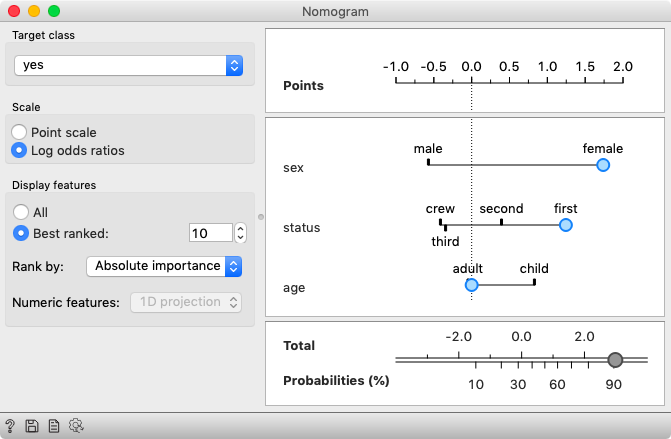
\includegraphics[scale=0.45]{graphics/ch-naive_bayes/nomogram.png}
    \caption{According to the probability theory individual contributions should be multiplied. Nomograms get around this by working in a log-space: a sum in the log-space is equivalent to multiplication in the original space. Therefore nomograms sum contributions (in the log-space) of all feature values and then convert them back to probability.}
\end{figure}

% Lesson 14: Classification Accuracy
\chapter{Classification Accuracy}
\label{ch:classification_accuracy}

Now that we know what classification trees are, the next question is what is the quality of their predictions. For beginning, we need to define what we mean by quality. In classification, the simplest measure of quality is classification \marginnote{$\mathrm{accuracy}=\frac{\# \{\mathrm{correct}\}}{\# \{\mathrm{all}\}}$} accuracy expressed as the proportion of data instances for which the classifier correctly guessed the value of the class. Let's see if we can estimate, or at least get a feeling for, classification accuracy with the widgets we already know.

\begin{wrapfigure}{o}{0.85\textwidth}
    \vspace{-0.5cm}
    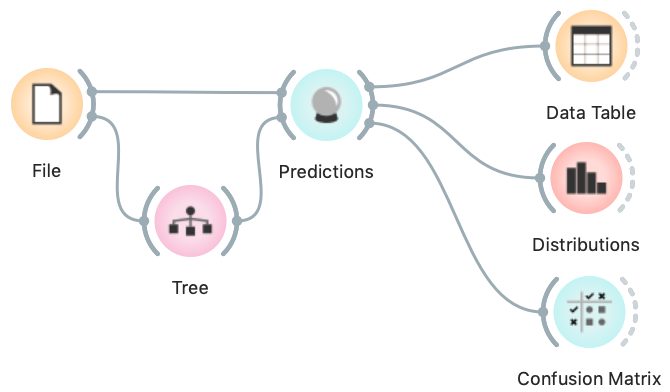
\includegraphics[scale=0.4]{graphics/ch-classification_accuracy/workflow.png}
\end{wrapfigure}

Let us try this schema with the \textit{iris} data set. The \widget{Predictions} widget outputs a data table augmented with a column that includes predictions. In the \widget{Data Table} widget, we can sort the data by any of these two columns, and manually select data instances where the values of these two features are different (this would not work on big data). Roughly, visually estimating the accuracy of predictions is straightforward in the \widget{Distribution} widget, if we set the features in view appropriately.

For precise statistics of correctly and incorrectly classified examples open the \widget{Confusion Matrix} widget.

\begin{figure*}[h]
    \centering
    \newcommand{\predictions}{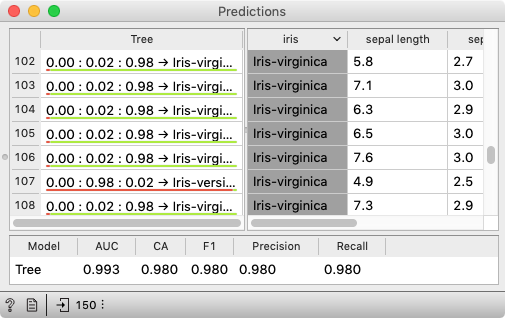
\includegraphics[scale=0.40]{graphics/ch-classification_accuracy/predictions2.png}}
    \newcommand{\distributions}{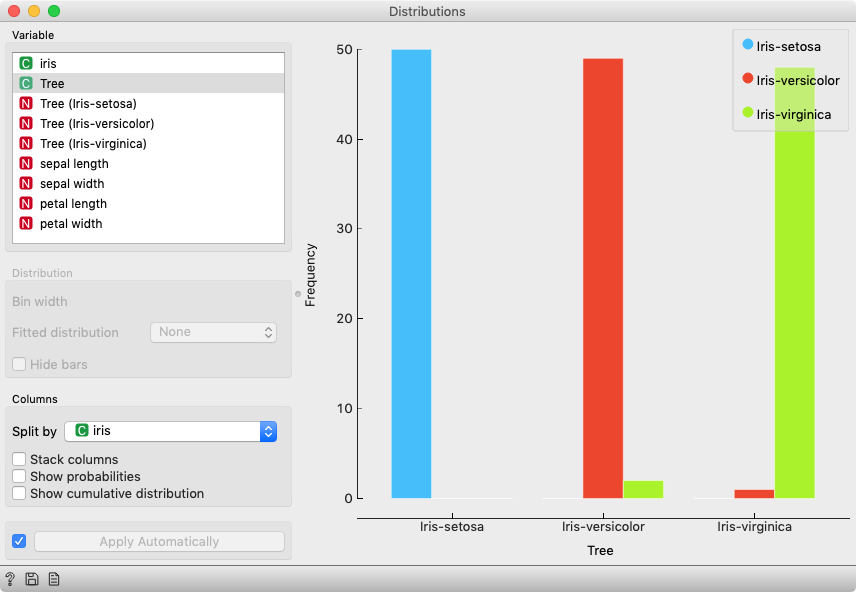
\includegraphics[scale=0.25]{graphics/ch-classification_accuracy/distributions.png}}
    \newcommand{\confusion}{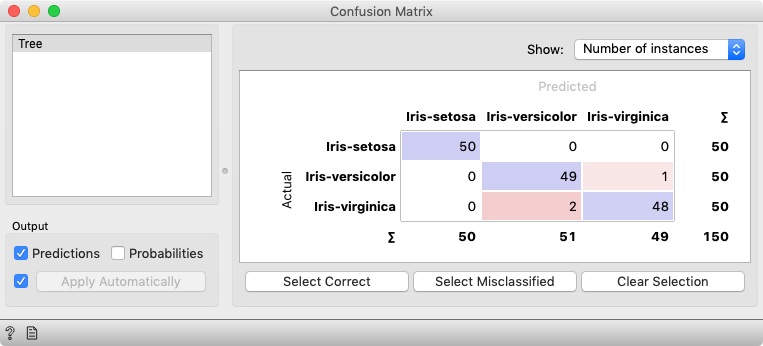
\includegraphics[scale=0.25]{graphics/ch-classification_accuracy/confusion.png}}
    \infinitewidthbox{
    \stackinset{r}{-0.35\linewidth}{b}{-0.05\linewidth}{\confusion}
    {\stackinset{r}{-0.35\linewidth}{b}{+0.15\linewidth}{\distributions}{\predictions}}\hspace{7cm}
    }
    \caption{The \widget{Confusion Matrix} shows 3 incorrectly classified examples, which makes the accuracy $(150-3)/150 = 98\%$.}
\end{figure*}

%Lesson 15: How to Cheat
\chapter{How to Cheat}
\label{ch:how_to_cheat}

\begin{wrapfigure}{o}{0.85\textwidth}
    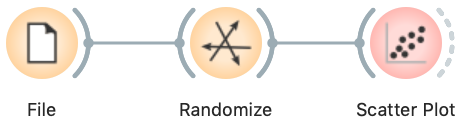
\includegraphics[scale=0.4]{graphics/ch-how_to_cheat/workflow-randomize.png}
\end{wrapfigure}

At this stage, \marginnote[-2cm]{This lesson has a strange title and it is not obvious why it was chosen. Maybe you, the reader, should tell us what does this lesson have to do with cheating.} the classification tree looks very good. There’s only one data point where it makes a mistake. Can we mess up the data set so bad that the trees will ultimately fail? Like, remove any existing correlation between features and the class? We can! There’s the \widget{Randomize} widget with class shuffling. Check out the chaos it creates in the \widget{Scatter Plot} visualization where there were nice clusters before randomization!

\begin{figure*}[h]
    \infinitewidthbox{
    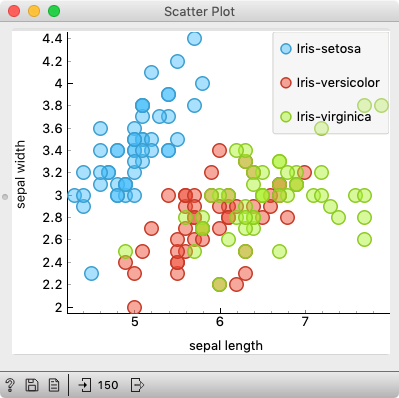
\includegraphics[scale=0.3]{graphics/ch-how_to_cheat/scatterplot_iris.png}
    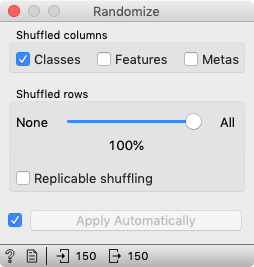
\includegraphics[scale=0.4]{graphics/ch-how_to_cheat/randomize100.png}
    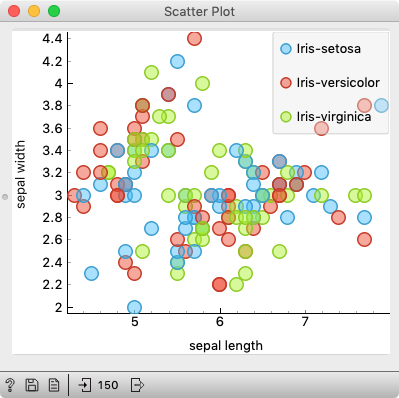
\includegraphics[scale=0.3]{graphics/ch-how_to_cheat/scatterplot_iris_random.png}
    }
    \caption{Left: scatter plot of the \textit{Iris} data set before randomization; right: scatter plot after shuffling 100\% of rows.}
\end{figure*}

Fine. There can be no classifier that can model this mess, right? Let’s make sure.

\begin{figure}[h]
    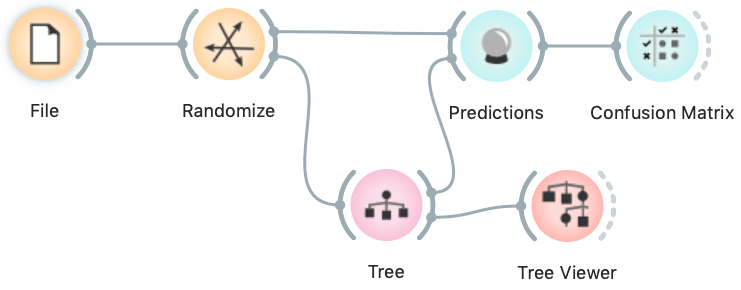
\includegraphics[scale=0.4]{graphics/ch-how_to_cheat/workflow_classification.png}
\end{figure}

\begin{wrapfigure}{o}{0.85\textwidth}
    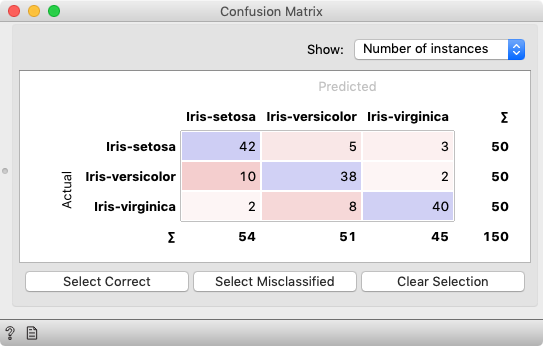
\includegraphics[scale=0.35]{graphics/ch-how_to_cheat/confusion_randomized.png}
\end{wrapfigure}

And the result? Here is a screenshot of the \widget{Confusion Matrix}.

Most unusual. Despite shuffling all the classes, which destroyed any connection between features and the class variable, about 80\% of predictions were still correct.

\clearpage

Can we further improve accuracy on the shuffled data? Let us try to change some properties of the induced trees: in the \widget{Tree} widget, disable all early stopping criteria.

\begin{figure}[h]
    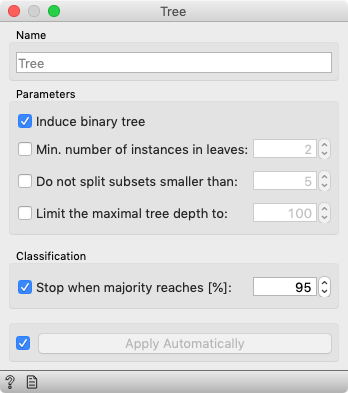
\includegraphics[scale=0.35]{graphics/ch-how_to_cheat/better_tree.png}
    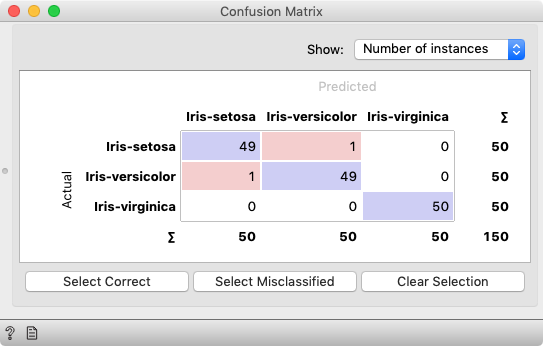
\includegraphics[scale=0.35]{graphics/ch-how_to_cheat/confusion_randomized_better.png}
    \caption{After we disable 2--4 check box in the \widget{Tree} widget, our classifier starts behaving almost perfectly.}
\end{figure}


Wow, almost no mistakes now. How is this possible? On a class-randomized data set?

\begin{wrapfigure}{o}{0.85\textwidth}
    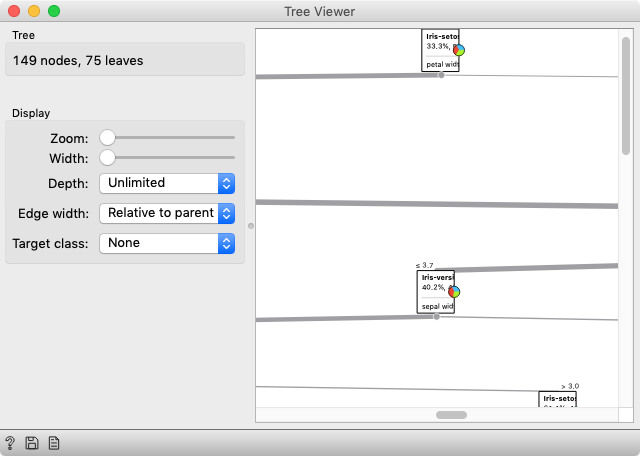
\includegraphics[scale=0.35]{graphics/ch-how_to_cheat/tree_viewer.png}
    \caption{In the build tree, there are 75 leaves. Remember, there are only 150 rows in the \textit{Iris} data set.}
\end{wrapfigure}

To find the answer to this riddle, open the \widget{Tree Viewer} and check out the tree. How many nodes does it have? Are there many data instances in the leaf nodes?

Looks like the tree just memorized every data instance from the data set. No wonder the predictions were right. The tree makes no sense, and it is complex because it simply remembered everything.

Ha, if this is so, if a classifier remembers everything from a data set but without discovering any general patterns, it should perform miserably on any new data set. Let us check this out. We will split our data set into two sets, training and testing, train the classification tree on the training data set and then estimate its accuracy on the test data set.

\begin{figure}[h]
    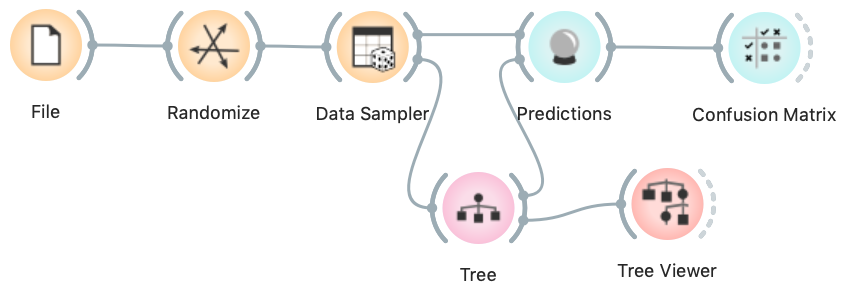
\includegraphics[scale=0.35]{graphics/ch-how_to_cheat/workflow_data_sampler.png}
    \caption{Connect the \widget{Data Sampler} widget carefully. The \widget{Data Sampler} splits the data to a sample and out-of-sample (so called remaining data). The sample was given to the \widget{Tree} widget, while the remaining data was handed to the \widget{Predictions} widget. Set the \widget{Data Sampler} so that the size of these two data sets is about equal.}
\end{figure}

Let’s check how the \widget{Confusion Matrix} looks after testing the classifier on the test data.

\begin{figure}[h]
    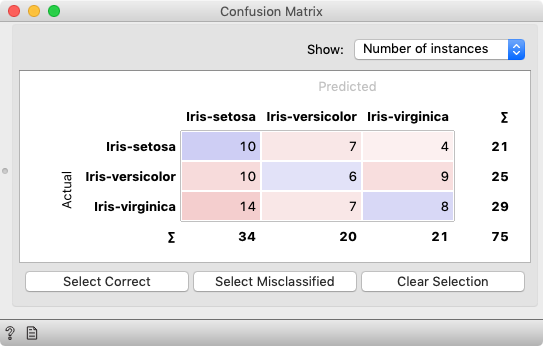
\includegraphics[scale=0.35]{graphics/ch-how_to_cheat/confusion_sampler.png}
    \caption{Confusion matrix if we estimate accuracy on a data set that was not used in learning.}
\end{figure}

The first two classes are a complete fail. The predictions for ribosomal genes are a bit better, but still with lots of mistakes. On the class-randomized training data our classifier fails miserably. Finally, just as we would expect.

We have just learned that we need to train the classifiers on the training set and then test it on a separate test set to really measure performance of a classification technique. With this test, we can distinguish between those classifiers that just memorize the training data and those that actually learn a general model.

Learning is not only memorizing. Rather, it is discovering patterns that govern the data and apply to new data as well. To estimate the accuracy of a classifier, we therefore need a separate test set. This estimate should not depend on just one division of the input data set to training and test set (here’s a place for cheating as well). Instead, we need to repeat the process of estimation several times, each time on a different train/test set and report on the average score.
% Lesson 16: Random Forests
\chapter{Random Forests}
\label{ch:random_forests}

\begin{wrapfigure}{o}{0.85\textwidth}
    \vspace{-0.5cm}
    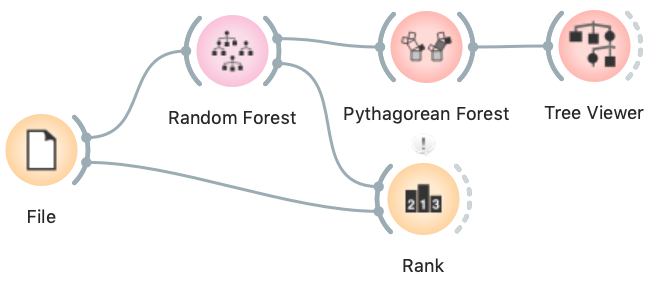
\includegraphics[scale=0.4]{graphics/ch-random_forests/workflow.png}
\end{wrapfigure}

Random forests, a modeling technique introduced in 2001, is still one of the best performing classification and regression techniques. Instead of building a tree by always choosing the a feature that seems to separate best at that time, it builds many trees in slightly random ways. Therefore the induced trees are different. For the final prediction the trees vote for the best class.

\begin{figure}[h]
    \centering
    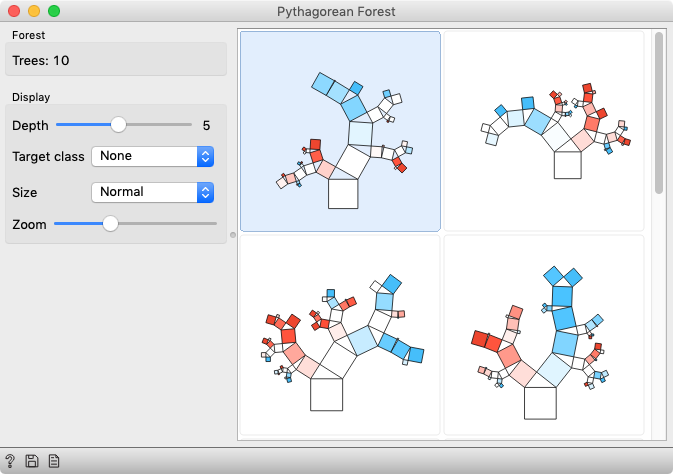
\includegraphics[scale=0.35]{graphics/ch-random_forests/pythagorean.png}
    \caption{The \widget{Pythagorean Forest} widget shows us how random the trees are. If we select a tree, we can observe it in a \widget{Tree Viewer}.}
\end{figure}

There are two sources of randomness: (1) training data is sampled with replacement, and (2) the best feature for a split is chosen among a subset of randomly chosen features.

Which features are the most important? The creators of random forests also defined a procedure for computing feature importances from random forests. In Orange, you can use it with the Rank widget.

\begin{figure}[h]
    \centering
    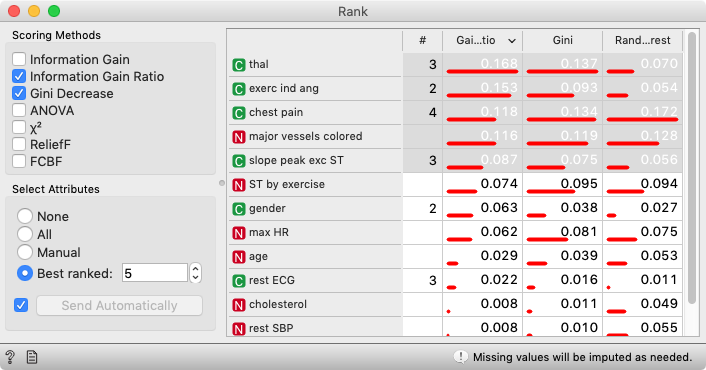
\includegraphics[scale=0.35]{graphics/ch-random_forests/rank.png}
    \caption{Feature importance according to two univariate measures (gain ratio and gini index) and random forests. Random forests also consider combinations of features when evaluating their importance. }
\end{figure}

% Lesson 17: Cross-Validation
\chapter{Cross-Validation}

\begin{wrapfigure}{o}{0.6\textwidth}
    \vspace{-0.5cm}
    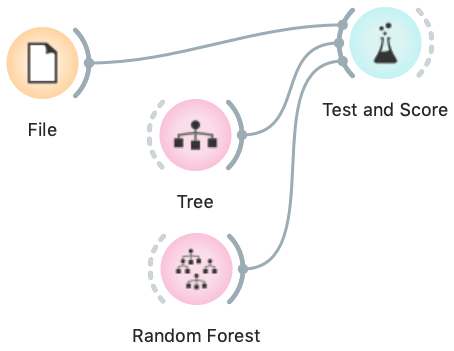
\includegraphics[scale=0.4]{graphics/ch-cross_validation/workflow.png}
\end{wrapfigure}

Estimating the accuracy may depend on a particular split of the data set. To increase robustness, we can repeat the measurement several times, each time choosing a different subset of the data for training. One such method is cross-validation. It is available in Orange through the \widget{Test and Score} widget.

Note that in each iteration, \widget{Test and Score} will pick a part of the data for training, learn the predictive model on this data using some machine learning method, and then test the accuracy of the resulting model on the remaining, test data set. For this, the widget will need on its input a data set from which it will sample the data for training and testing, and a learning method which it will use on the training data set to construct a predictive model. In Orange, the learning method is simply called a learner. Hence, \widget{Test and Score} needs a learner on its input. \marginnote{For geeks: a learner is an object that, given the data, outputs a classifier. Just what \widget{Test and Score} needs.}

This is another way to use the \widget{Tree} widget. In the workflows from the previous lessons we have used another of its outputs, called \textit{Model}; its construction required data. This time, no data is needed for \widget{Tree}, because all that we need from it is a \textit{Learner}.

\begin{figure}[h]
    \centering
    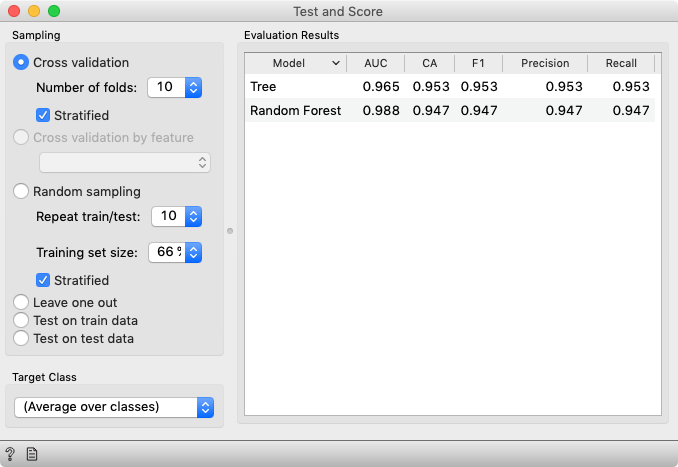
\includegraphics[scale=0.4]{graphics/ch-cross_validation/test_and_score.png}
    \caption{Cross validation splits the data sets into, say, 10 different non-overlapping subsets we call folds. In each iteration, one fold will be used for testing, while the data from all other folds will be used for training. In this way, each data instance will be used for testing exactly once.}
\end{figure}

In the \widget{Test and Score} widget, the second column, CA, stands for classification accuracy, and this is what we really care for for now.
% Lesson 18: Hierarchical Clustering
\chapter{Hierarchical Clustering}
\label{ch:hierarchical_clustering}

Say that we are interested in finding clusters in our data. That is, we would like to identify groups of data instances that are close together, similar to each other. Consider a simple, two-featured data set (see the side note) and plot it in the Scatter Plot. How many clusters do we have? What defines a cluster? Which data instances should belong to the same cluster? How does the clustering algorithm actually work?

\begin{marginfigure}
    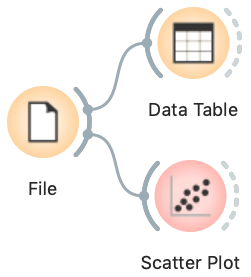
\includegraphics[scale=0.4]{graphics/ch-hierarchical_clustering/workflow_scatterplot.png}
    \caption{We will introduce clustering with a simple data set on students and their grades in English and Algebra.
Load the data set from \url{http://file.biolab.si/text/grades.tab}.}
\end{marginfigure}

First, we need to define what we mean by ``similar''. We will assume that all our data instances are described (profiled) with continuous features. One simple measure of similarity is the Euclidean distance. So, we would like to group data instances with small Euclidean distances.

\begin{figure*}[h]
    \vspace{1cm}
    \centering
    \infinitewidthbox{
    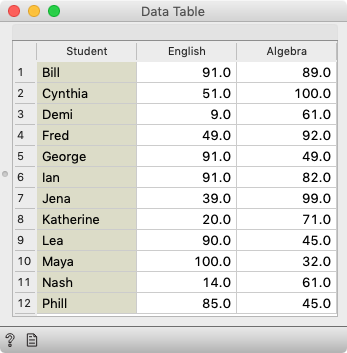
\includegraphics[scale=0.4]{graphics/ch-hierarchical_clustering/grades_table.png}
    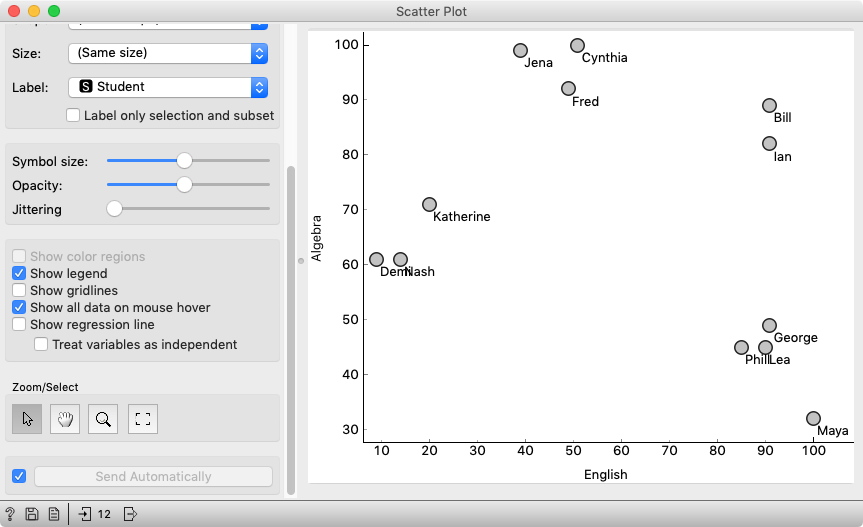
\includegraphics[scale=0.4]{graphics/ch-hierarchical_clustering/grades_scatterplot.png}
    }
    \caption{There are different ways to measure the similarity between clusters. The estimate we have described is called average linkage. We could also estimate the distance through the two closest points in each clusters (single linkage), or through the two points that are furthest away (complete linkage).}
\end{figure*}

Next, we need to define a clustering algorithm. Say that we start with each data instance being its own cluster, and then, at each step, we join the clusters that are closest together. We estimate the distance between the clusters with, say, the average distance between all their pairs of data points. This algorithm is called hierarchical clustering.

\clearpage

One possible way to observe the results of clustering on our small data set with grades is through the following workflow:

\begin{marginfigure}
    \centering
    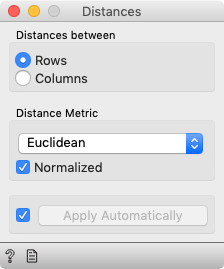
\includegraphics[scale=0.4]{graphics/ch-hierarchical_clustering/distances.png}
\end{marginfigure}

\begin{figure}[h]
    \centering
    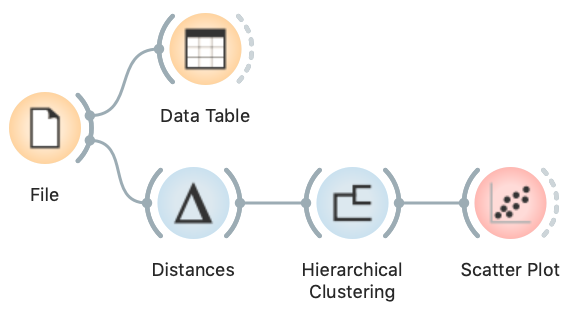
\includegraphics[scale=0.4]{graphics/ch-hierarchical_clustering/workflow_clustering.png}
    \caption{$\;$} % empty caption for proper pagesetting
\end{figure}

Couldn’t be simpler. Load the data, measure the distances, use them in hierarchical clustering, and visualize the results in a scatter plot. The \widget{Hierarchical Clustering} widget allows us to cut the hierarchy at a certain distance score and output the corresponding clusters:

\begin{figure*}[h]
    \centering
    \newcommand{\clustering}{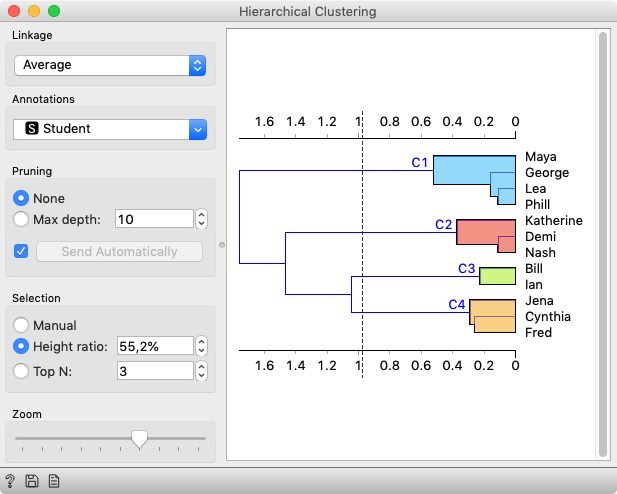
\includegraphics[scale=0.4]{graphics/ch-hierarchical_clustering/hierarchical_clustering.png}}
    \newcommand{\plot}{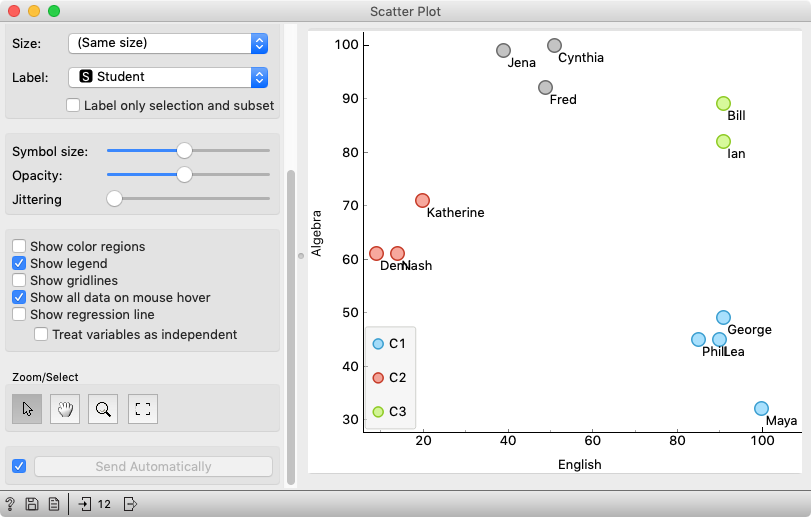
\includegraphics[scale=0.4]{graphics/ch-hierarchical_clustering/scatterplot_clustered.png}}
    \infinitewidthbox{
    \stackinset{r}{-0.5\linewidth}{t}{+0.3\linewidth}{\plot}{\clustering}\hspace{8cm}
    }
\end{figure*}

% Lesson 19: Animal Kingdom
\chapter{Animal Kingdom}
\label{ch:animal_kingdom}

\begin{marginfigure}
    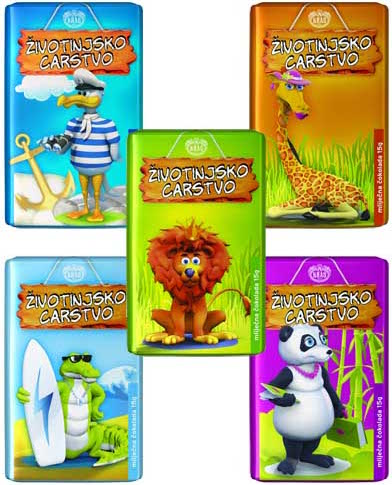
\includegraphics[width=5cm]{graphics/ch-animal_kingdom/kras_zivotinjsko_carstvo.jpg}
\end{marginfigure}

Your lecturers spent a substantial part of their youth admiring a particular Croatian chocolate called Animal Kingdom. Each chocolate bar came with a card---a drawing of some (random) animal, and the associated album made us eat a lot of chocolate.

Funny stuff was we never understood the order in which the cards were laid out in the album. We later learned about taxonomy, but being more inclined to engineering we never mastered learning it in our biology classes. Luckily, there’s data mining and the idea that taxonomy simply stems from measuring the distance between species.

\begin{wrapfigure}{o}{0.8\textwidth}
    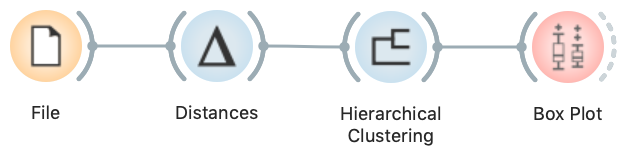
\includegraphics[scale=0.4]{graphics/ch-animal_kingdom/workflow.png}
    \caption{Hierarchical clustering works fast for smaller data sets. But for bigger ones it fails. Simply, it cannot be used. Why?}
\end{wrapfigure}

Here we use zoo data (from the documentation data sets) with attributes that report on various features of animals (has hair, has feathers, lays eggs). We measure the distance and compute the clustering. Animals in this data set are annotated with type (mammal, insect, bird, and so on). It would be cool to know if the clustering re-discovered these groups of animals.

To split the data into clusters, let us manually set a threshold by dragging the vertical line left or right in the visualization. Can you say what is the appropriate number of groups?

\begin{figure*}[h]
    \centering
    \newcommand{\clustering}{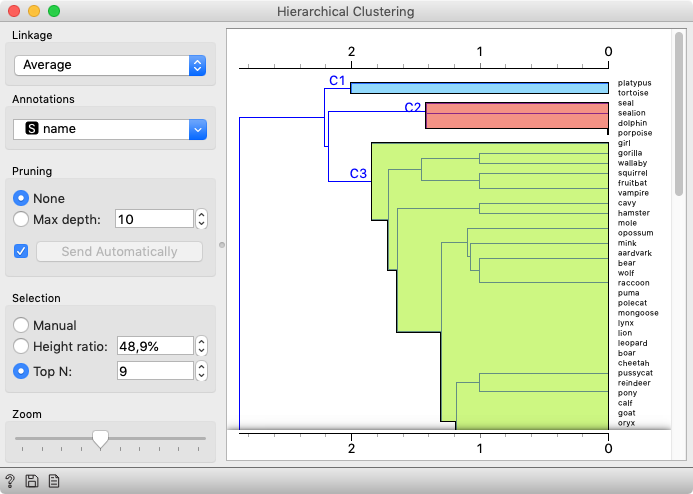
\includegraphics[scale=0.35]{graphics/ch-animal_kingdom/clustering.png}}
    \newcommand{\plot}{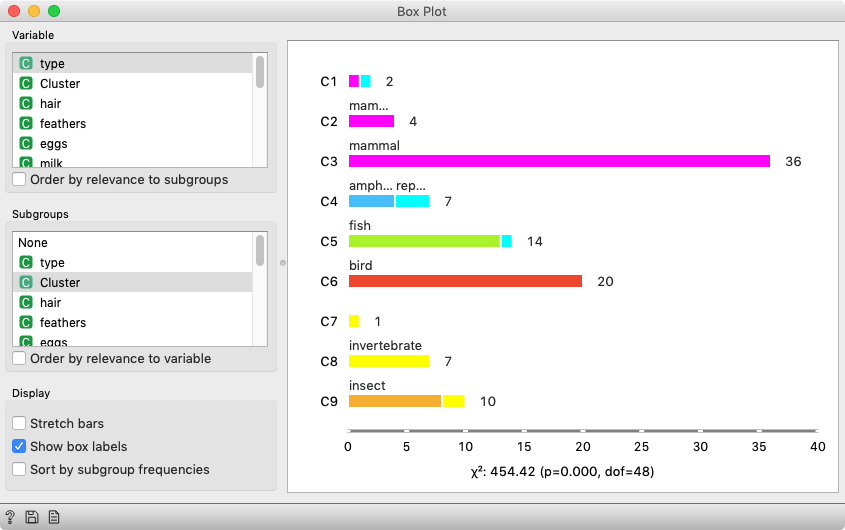
\includegraphics[scale=0.35]{graphics/ch-animal_kingdom/boxplot.png}}
    \infinitewidthbox{
    \stackinset{r}{-0.5\linewidth}{t}{+0.1\linewidth}{\plot}{\clustering}\hspace{8cm}
    }
    \caption{What is wrong with those mammals? Why can't they be in one single cluster? Two reasons. First, they represent 40\% of the data instances. Second, they include some weirdos. Who are they?}
\end{figure*}


% Lesson 20: Classification of Spectra
\chapter{Classification of Spectra}
\label{ch:spectra_classification}

\begin{wrapfigure}{o}{0.82\textwidth}
    \centering
    \vspace{-3.4cm}
    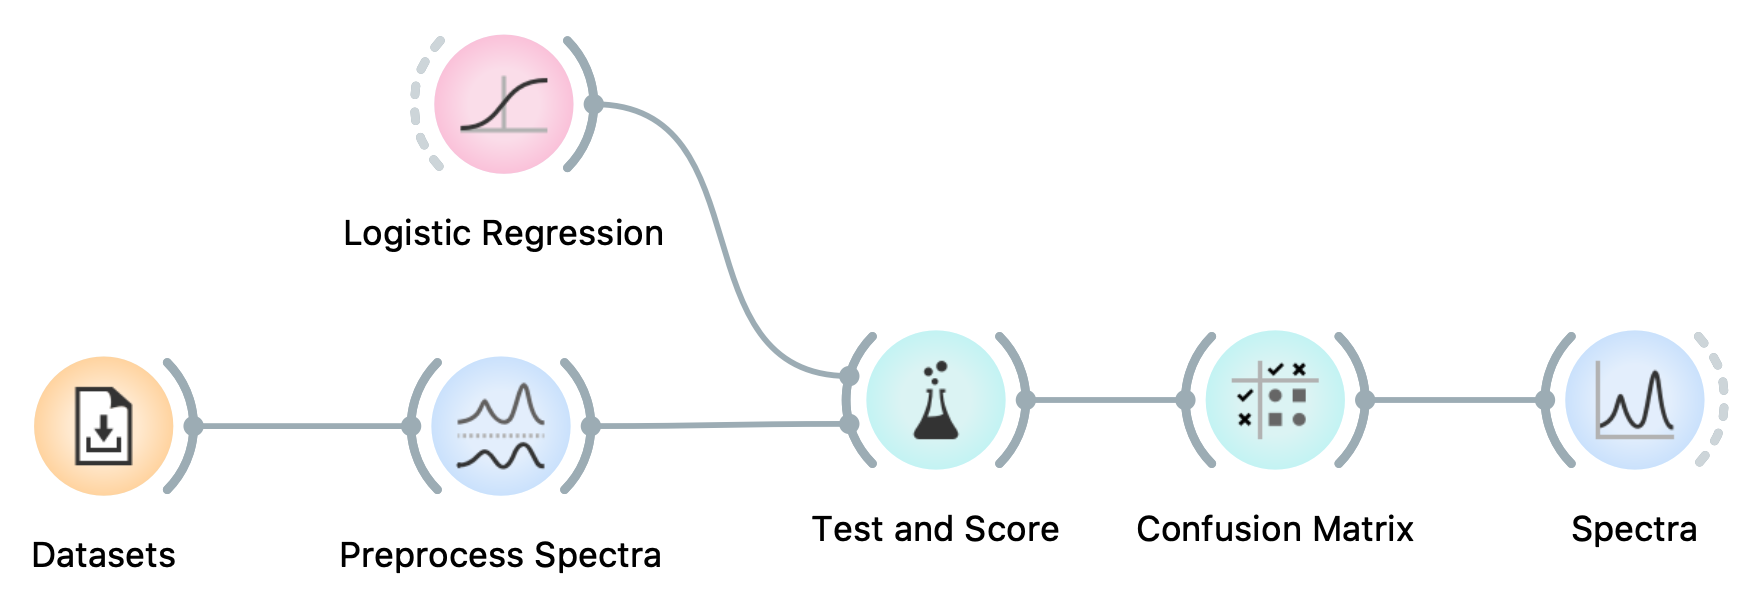
\includegraphics[width=0.95\textwidth]{graphics/ch-spectra_classification/sp_classification-fig1.png}
    \label{fig:spectra_classification-fig1}
\end{wrapfigure}


Let’s open the collagen data set again and see how well can logistic regression predict its four classes. Straightforward, right? Connect \widget{Datasets}, \widget{Logistic Regression}, \widget{Predictions}, \widget{Confusion Matrix} and that's it. We would also like to do some spectral processing (we will only keep the columns for wavenumbers between 1500\wn and 1800\wn).

\begin{figure}[h]
\hspace{-1cm}\stackinset{r}{-0.7\linewidth}{t}{+0.25\linewidth}
  {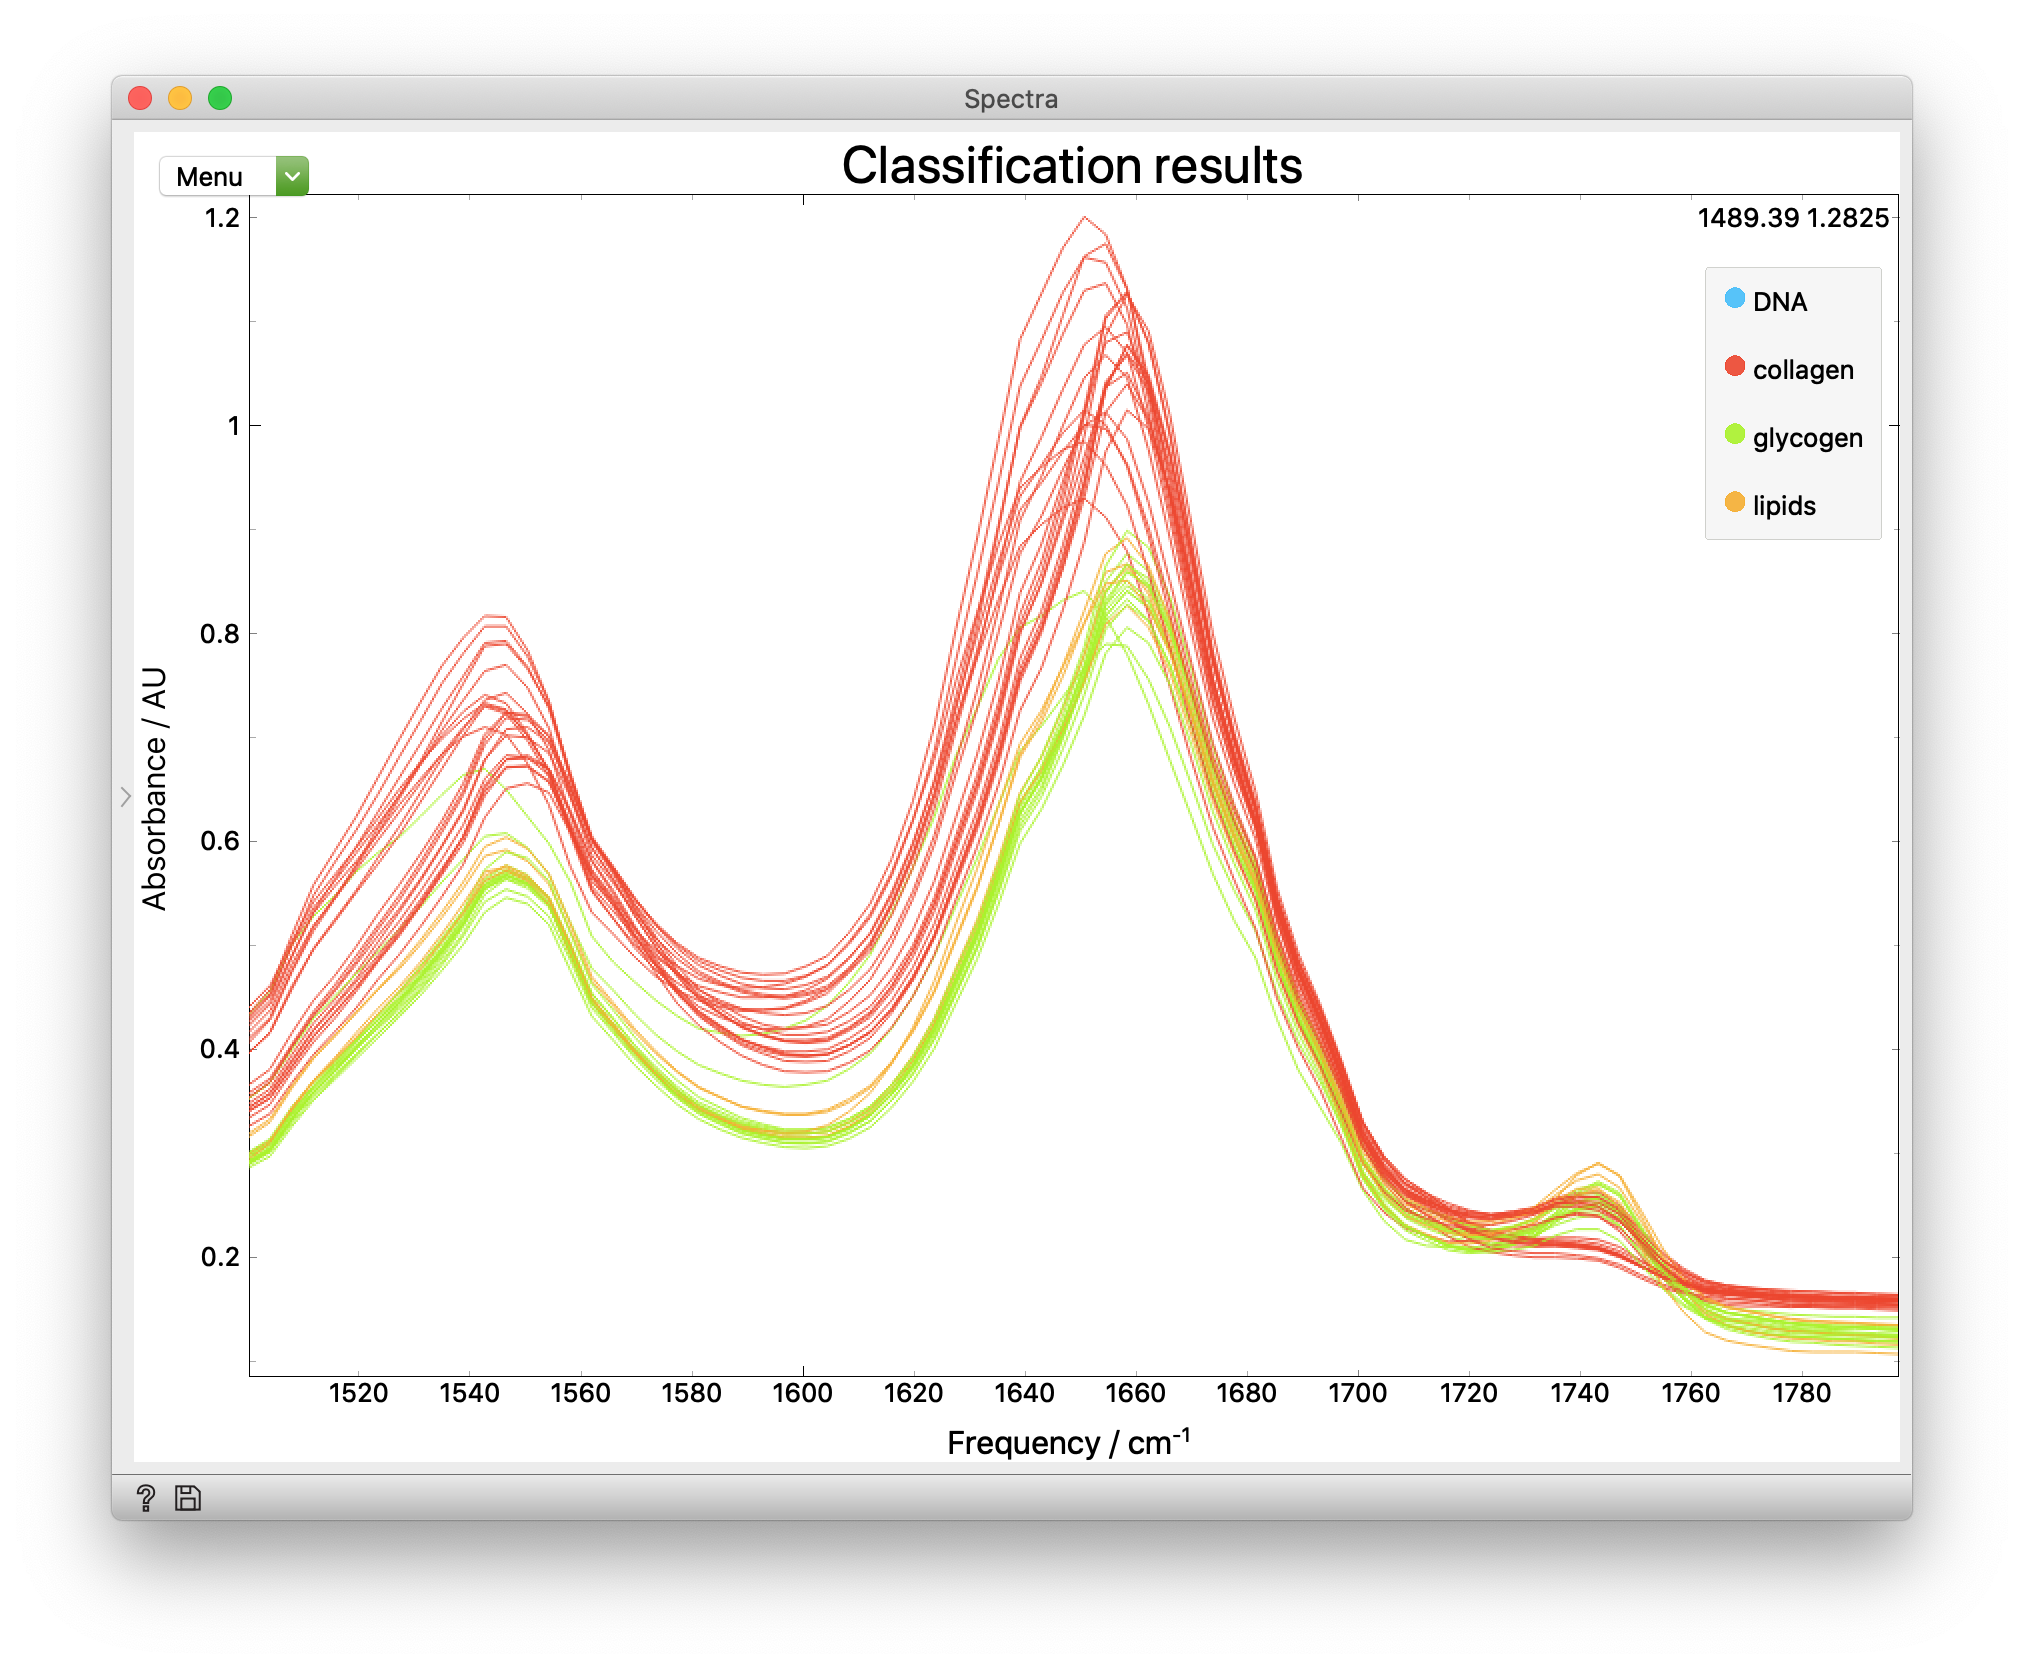
\includegraphics[scale=0.35]{graphics/ch-spectra_classification/sp_classification-fig2b.png}}
  {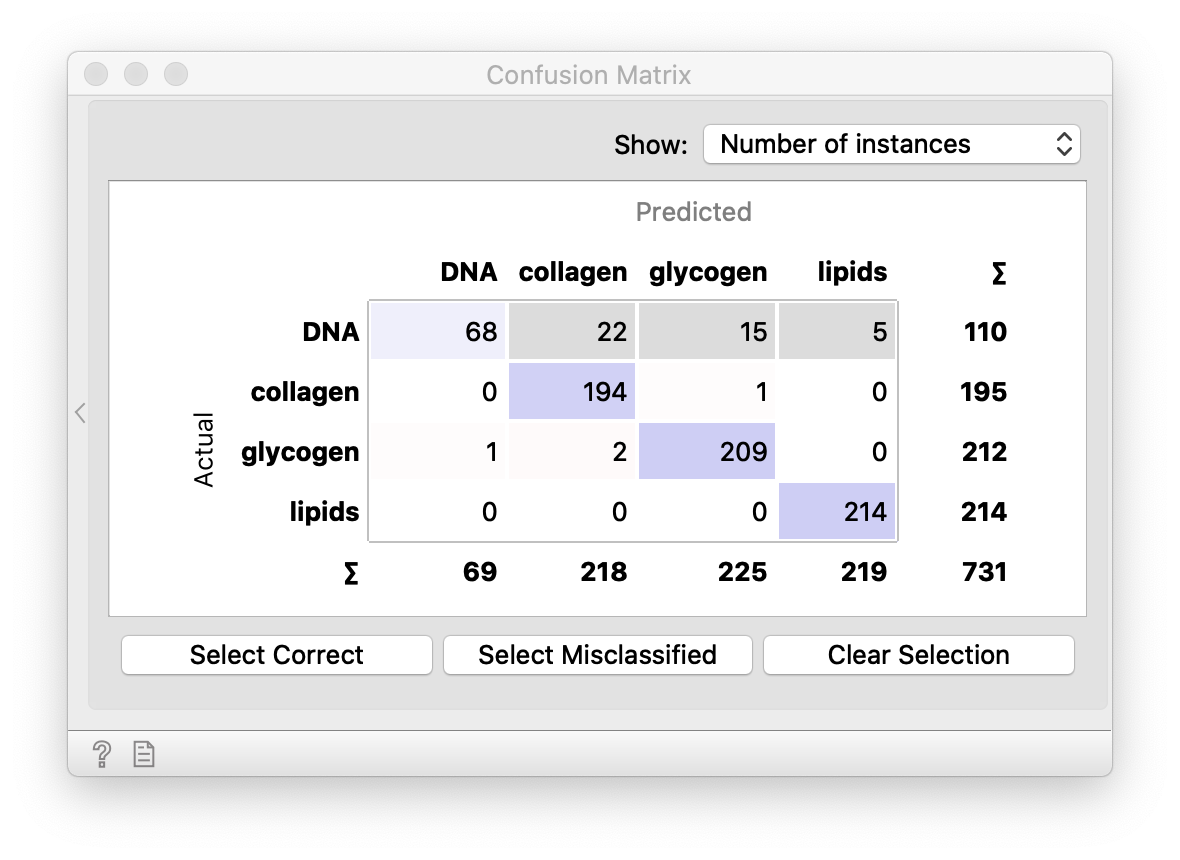
\includegraphics[scale=0.45]{graphics/ch-spectra_classification/sp_classification-fig2a_.png}}
  \caption{The \widget{Spectra} widget shows wrong predictions for the DNA class.}
  \label{fig:spectra_classification-fig2}
\end{figure}

Let’s not forget that it is pointless to predict for the same data as we used for learning. We could either  use a \widget{Data Sampler} and connect its Sample output to \widget{Preprocess Spectra} and Remaining output to \widget{Predictions}, or obtain predictions from the \widget{Test and Score} widget.
\widget{Confusion Matrix} now shows the mistakes of the model (scored with cross-validation). We can select them and inspect them further in a \widget{Spectra} widget. Here we colored them by the predicted class (see the Menu). 

\begin{wrapfigure}{o}{1.1\textwidth}
  \centering
  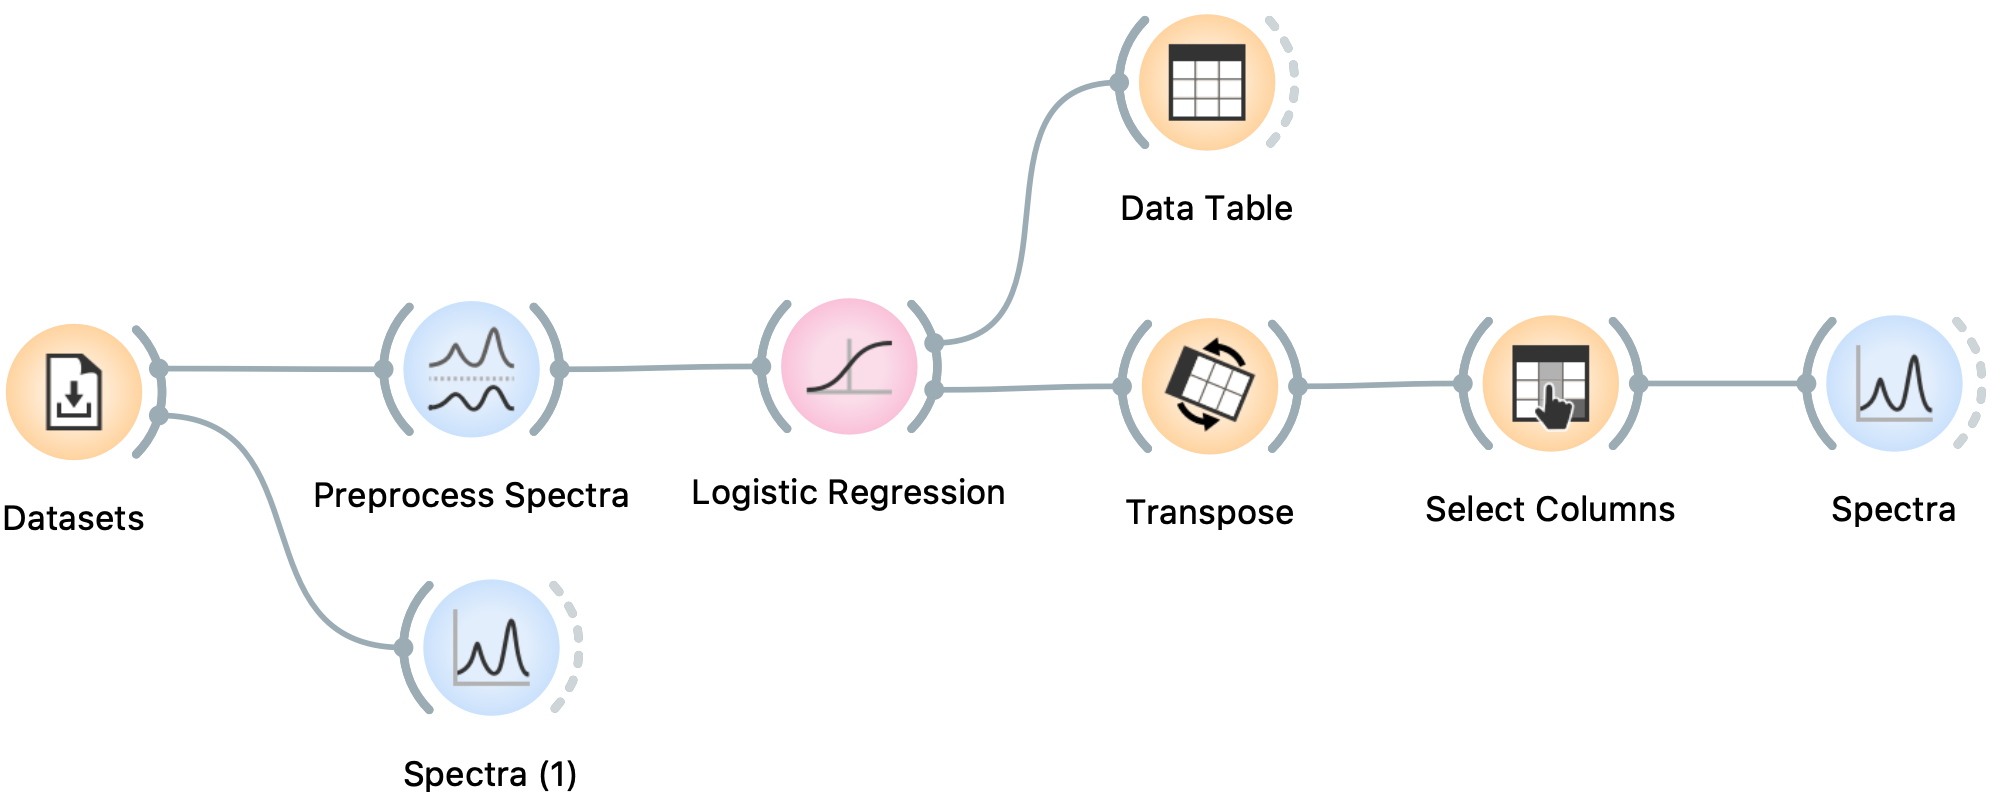
\includegraphics[width=1.1\textwidth]{graphics/ch-spectra_classification/sp_classification-fig3.png}%
  \label{fig:spectra_classification-fig3}
\end{wrapfigure}
But how does the model make its decisions? We already inspected a different model, classification tree, where each node represents a decision on a value of a column.  \widget{Logistic regression} works differently. On the training data it computes weights for all columns (wavelengths), which are then used for prediction, where values are multiplied with weights. To see the weights, connect \widget{Logistic Regression} to a \widget{Data Table}. 

\begin{wrapfigure}{o}{0.9\textwidth}
%  \centering
  \vspace{-0.7cm}
  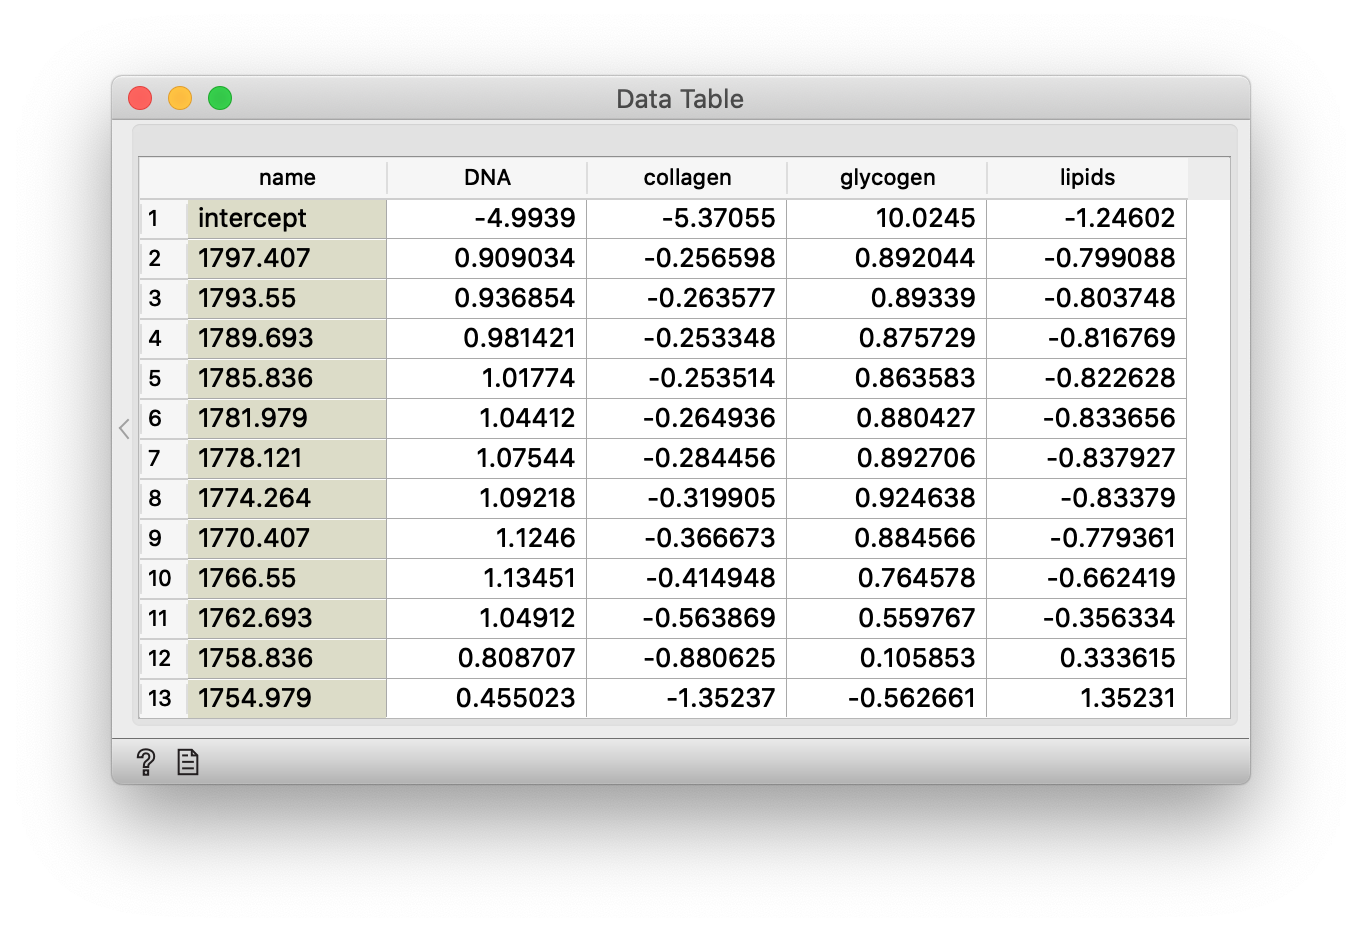
\includegraphics[width=0.9\textwidth]{graphics/ch-spectra_classification/sp_classification-fig4.png}
  \label{fig:spectra_classification-fig4}
\end{wrapfigure}
We get a table that is hard to understand. What if we visualize it? First, \widget{Transpose} the data. Then, use \widget{Select Columns} to make the visualization prettier: in the widget remove the intercept.

Now, open \widget{Logistic Regression} and try changing its parameters. Observe the effect on the weights.

\begin{figure}[h]
\hspace{-1cm}\stackinset{r}{0\linewidth}{t}{-0.22\linewidth}
  {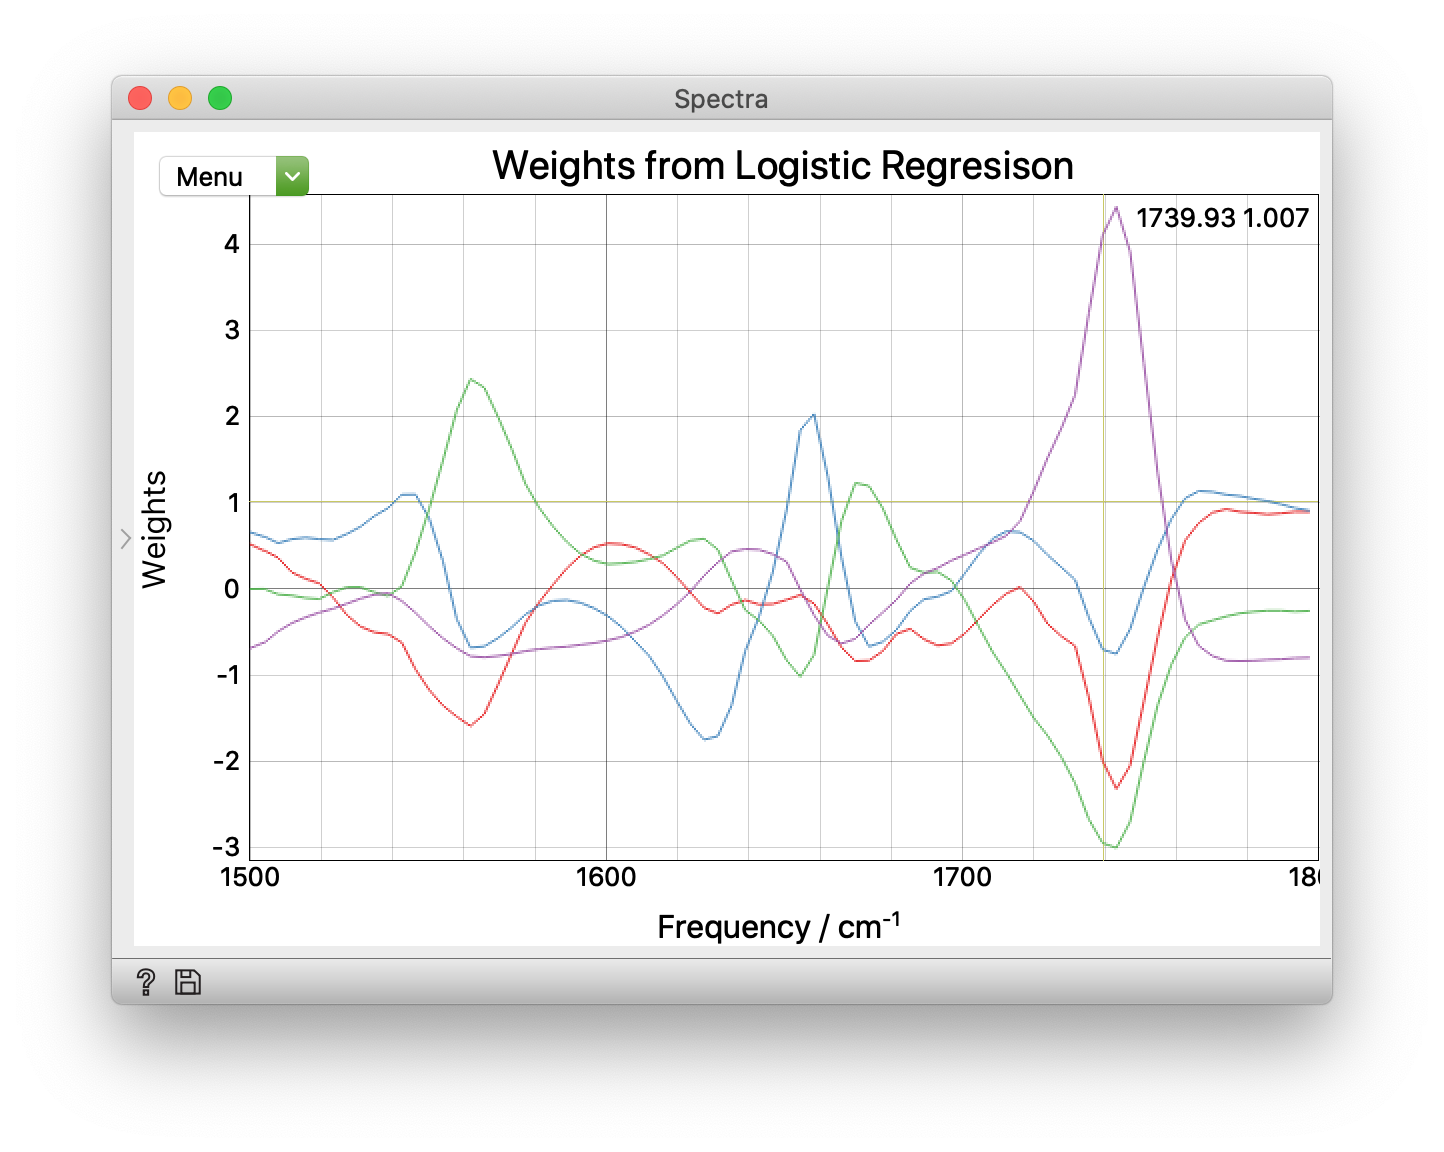
\includegraphics[scale=0.35]{graphics/ch-spectra_classification/sp_classification-fig5a.png}}
  {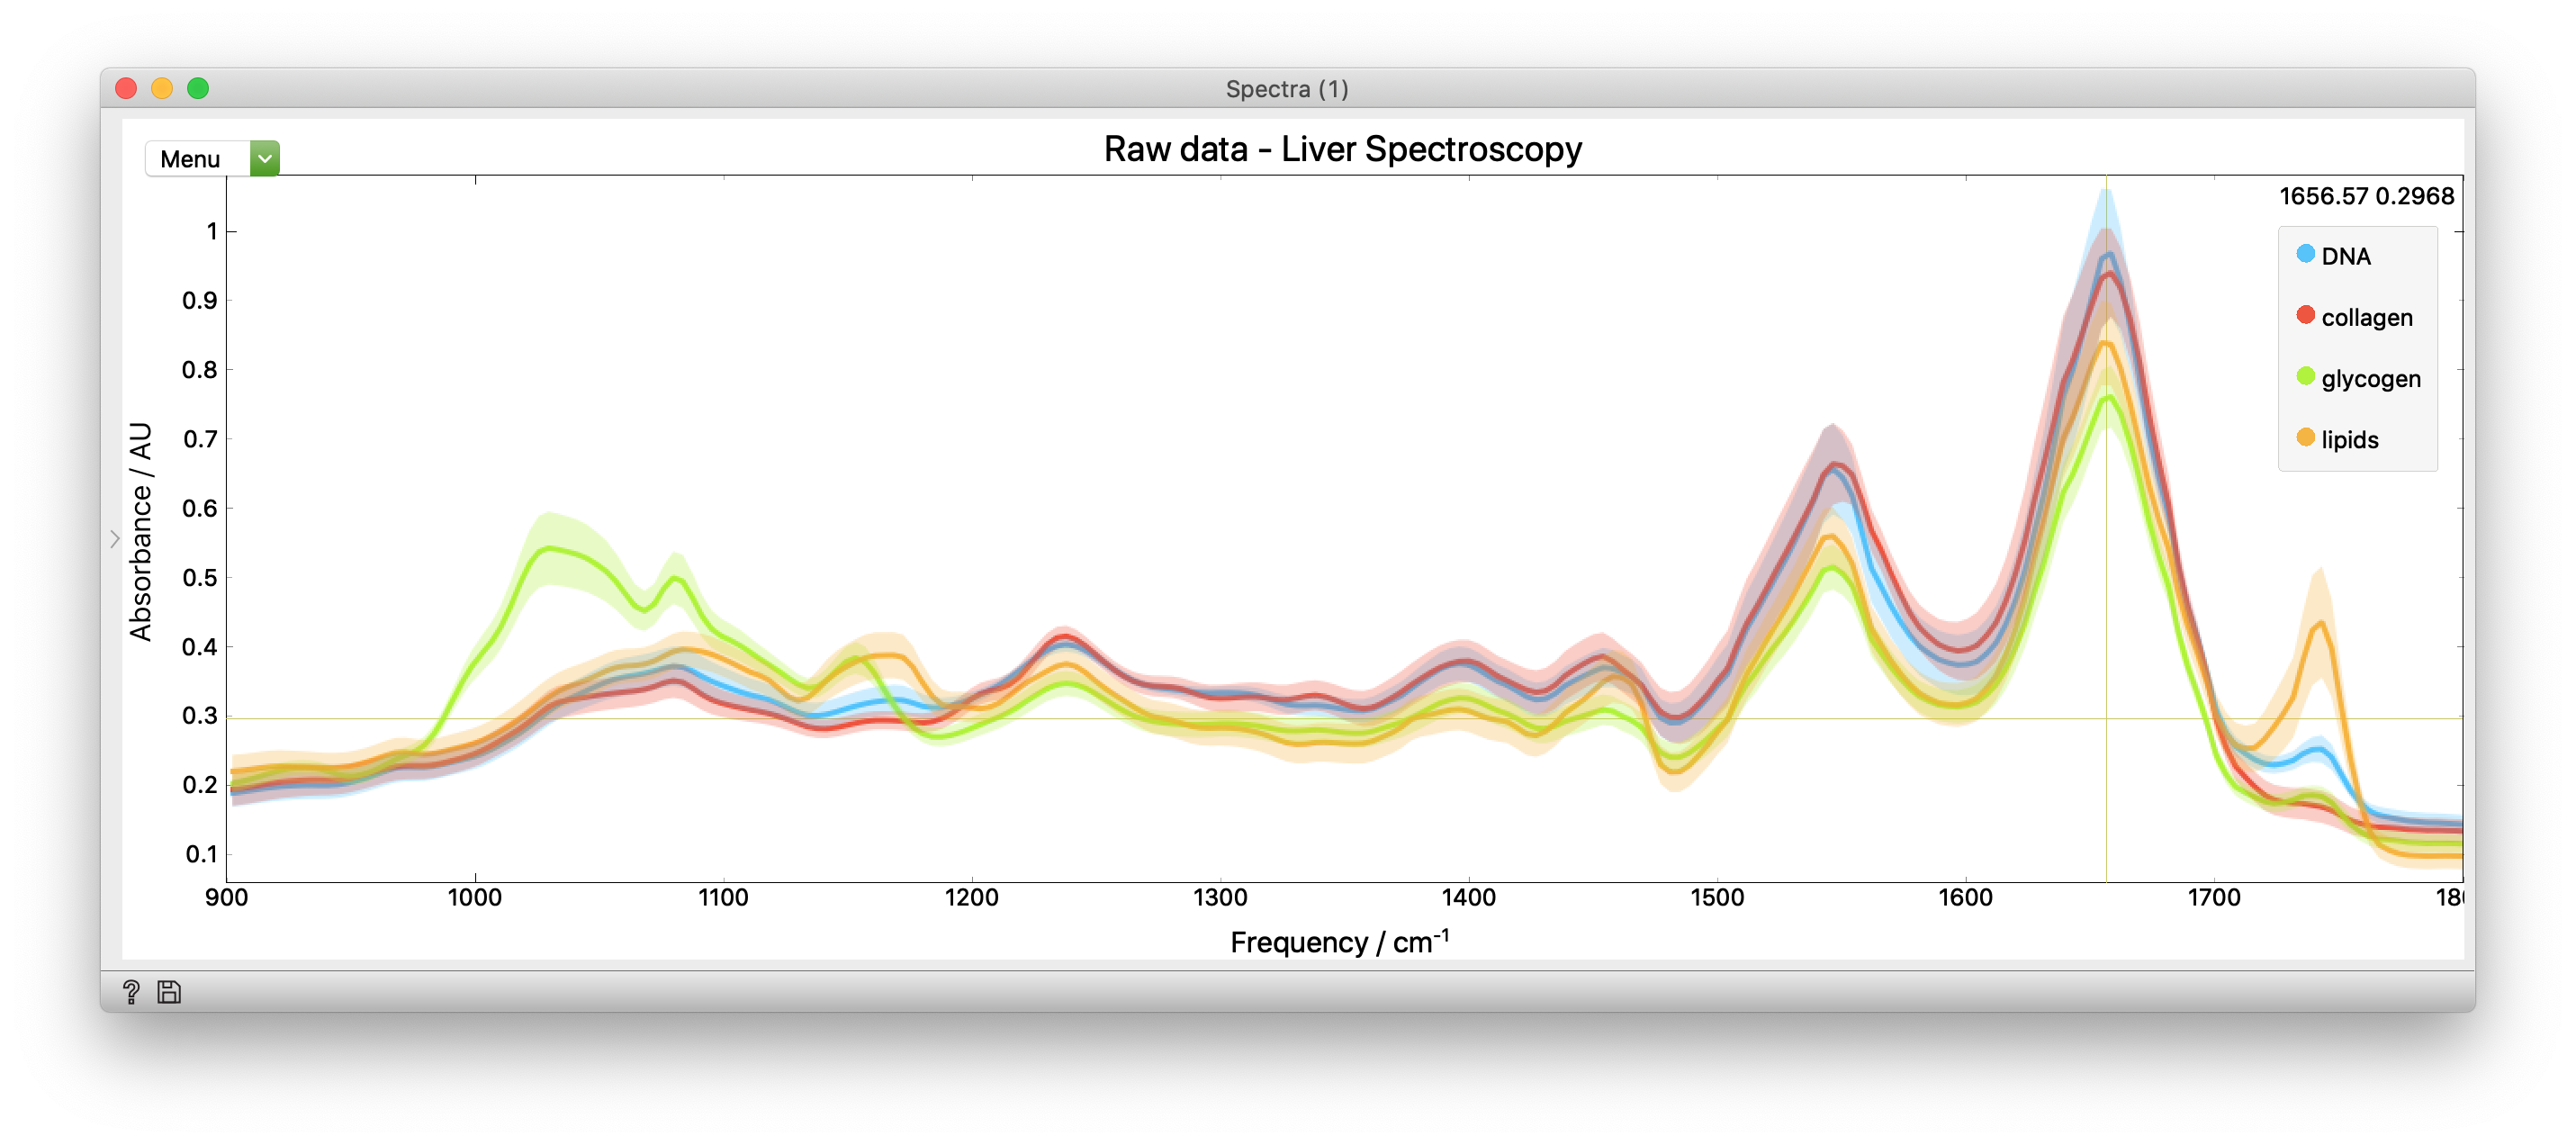
\includegraphics[scale=0.35]{graphics/ch-spectra_classification/sp_classification-fig5b.png}}
  \label{fig:spectra_classification-fig5}
\end{figure}

%TODO Marko % Lesson 21: New and Different Test Data
% Lesson 22: Clustering Spectral Images
\chapter{Clustering Spectral Images}
\label{ch:spectra_image_clustering}

\begin{wrapfigure}{o}{0.63\textwidth}
    \centering
    \vspace{-3.3cm}
    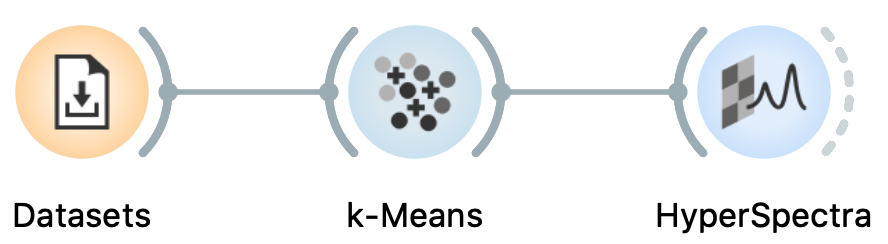
\includegraphics[width=0.75\textwidth]{graphics/ch-spectra_image_clustering/sp_image_clustering-fig1.png}
    \label{fig:spectra_image_clustering-fig1}
\end{wrapfigure}

We have already seen hierarchical clustering. Another clustering algorithm, k-Means, is much faster for data with lots of rows, like images, which contain a row (a spectrum) for each pixel. Still, for the liver-cirrhosis data, both approaches are fast. Here, we use \widget{k-Means} with k=3 clusters. 

\begin{figure}[h]
\vspace{-0.5cm}
\hspace{-1cm}\stackinset{r}{-1.15\linewidth}{t}{0.025\linewidth}
  {\includegraphics[scale=0.33]{graphics/ch-spectra_image_clustering/sp_image_clustering-fig2b.png}}
  {\includegraphics[scale=0.55]{graphics/ch-spectra_image_clustering/sp_image_clustering-fig2a.png}}
%  \caption{The \widget{Spectra} widget shows wrong predictions for the DNA class.}
  \label{ffig:spectra_image_clustering-fig2}
\end{figure}



\begin{wrapfigure}{o}{1.1\textwidth}
  \centering
  \includegraphics[width=1.1\textwidth]{graphics/ch-spectra_image_clustering/sp_image_clustering-fig3.png}%
  \label{fig:spectra_image_clustering-fig3}
\end{wrapfigure}
We see no meaningful clusters. Therefore, we need to preprocess the data. If we do it well, we see that a cluster corresponds to the background. We could remove it with the Select Rows widget.

\begin{wrapfigure}{o}{0.9\textwidth}
%  \centering
  \vspace{-0.5cm}
  \includegraphics[width=0.9\textwidth]{graphics/ch-spectra_classification/sp_classification-fig4.png}
  \label{fig:spectra_classification-fig4}
\end{wrapfigure}

%TODO Feri % Lesson 23: PCA with Spectral Images
%TODO Feri % Lesson 24: Classification on Hyperspectral Images
%TODO Feri % Lesson 25: Preprocessing with EMSC
%TODO Feri % Lesson 26: Adding Annotations
% Lesson 27: Visualizing similarities based on various metrics (Neighbors widget)
\chapter{Visualize spectral distances}
\label{ch:visualize-spectral-distances}

\begin{wrapfigure}{o}{0.65\textwidth}
	\vspace{-1.5 cm}
    \includegraphics[scale=0.6]{graphics/ch-visualize_spectral_distances/ch-visualize_spectral_distances-fig1.png}
\end{wrapfigure}

Let's consider a spectrum, or any other data entry for that matter, as a point in a multidimensional space. We can define distance metrics between these points and visualize the distance values from one another or from a selected reference point or reference spectrum. By doing so, we can explore how similar our measurements are to a selected reference. We can do this on a series of spectra or even on hyperspectral maps!

If you build the workflow shown above this paragraph in \mutation\ you will be able to explore various distance metrics. First, let's use the \textit{'Liver cirrhosis - spectral image'} dataset provided by the \widget{Datasets} widget, then calculate the \textit{Euclidean distances} from the average spectrum with the \widget{Neighbors} widget and visualize them in \widget{Hyperspectra}. 

\medskip
Can you reproduce the results below? Pay attention to the color scheme.

\begin{figure*}[h]
\centering
\infinitewidthbox{
  \stackinset{r}{-0.5\linewidth}{t}{+0.1\linewidth}
  {\includegraphics[scale=0.4]{graphics/ch-visualize_spectral_distances/ch-visualize_spectral_distances-fig3.png}}
  {\includegraphics[scale=0.6]{graphics/ch-visualize_spectral_distances/ch-visualize_spectral_distances-fig2.png}}
  \hspace{8cm}
  }
%\caption{Try changing the parameters!}

\end{figure*}

Explore different distance metrics, inspect distances in a \widget{Data Table} widget. Don't forget, you can select points on the top map and see the corresponding spectra on the bottom in \widget{Hyperspectra}. 

% I would like to have a special environment called notes for example that we can switch on or off to print or hide lecturer notes.
\lecnotes{Possibility for discussion of the general mathematical properties of distance functions. See \url{https://en.wikipedia.org/wiki/Metric_(mathematics)}}
%%
% The back matter contains appendices, bibliographies, indices, glossaries, etc.
\backmatter

\bibliography{sample-handout}
\bibliographystyle{plainnat}


\printindex

\end{document}
